% ============================================================================
%  Embedded Systems Course Project Report
%  40 MHz Dual-Range Auto-Switching Digital Frequency Meter with Android Telemetry
%  Alexandria University | Supervisor: Dr. Housam Abdelbaki
%
%  HOW TO COMPILE:
%    - Recommended: Upload FreqMeter_Report_Overleaf.zip (or the docs/ folder)
%      to Overleaf and compile with pdfLaTeX.
%    - Locally: pdflatex FreqMeter_Report.tex (run twice for TOC & references).
%
%  GITHUB REPOSITORY:
%    - https://github.com/m7mdelsayegh/frequency_meter
% ============================================================================
\documentclass[11pt,a4paper]{article}

% --- Encoding & Fonts ---
\usepackage[utf8]{inputenc}
\usepackage[T1]{fontenc}
\usepackage{lmodern}
\usepackage{microtype}

% --- Page Layout & Headers ---
\usepackage[a4paper, margin=2.3cm, top=2.6cm, bottom=2.5cm]{geometry}
\usepackage{fancyhdr}
\usepackage{titlesec}
\usepackage{parskip}
\setlength{\parindent}{0pt}
\setlength{\parskip}{6pt}

% --- Math & Units ---
\usepackage{amsmath, amssymb}

% --- Graphics, Figures, Tables ---
\usepackage{graphicx}
\usepackage{float}
\usepackage{subcaption}
\usepackage{booktabs}
\usepackage{tabularx}
\usepackage{array}
\usepackage{multirow}
\usepackage{enumitem}
\usepackage[labelfont=bf, font=small]{caption}

% --- Colors & Boxes ---
\usepackage[dvipsnames, table]{xcolor}
\definecolor{NavyPrimary}{HTML}{1B365D}
\definecolor{TealAccent}{HTML}{2B6CB0}
\definecolor{SoftBg}{HTML}{F4F7FA}
\definecolor{BorderGray}{HTML}{CBD5E0}
\definecolor{CodeBg}{HTML}{F8FAFC}
\definecolor{CodeComment}{HTML}{5C6B73}
\definecolor{CodeKeyword}{HTML}{1D4ED8}
\definecolor{CodeString}{HTML}{B91C1C}

\usepackage[most]{tcolorbox}

% --- TikZ for Block Diagrams & Flowcharts ---
\usepackage{tikz}
\usetikzlibrary{shapes.geometric, arrows.meta, positioning, fit, backgrounds, calc}

% --- Source Code Listings ---
\usepackage{listings}
\lstset{
    backgroundcolor=\color{CodeBg},
    basicstyle=\ttfamily\footnotesize,
    breaklines=true,
    breakatwhitespace=true,
    captionpos=b,
    commentstyle=\color{CodeComment}\itshape,
    keywordstyle=\color{CodeKeyword}\bfseries,
    stringstyle=\color{CodeString},
    frame=single,
    rulecolor=\color{BorderGray},
    numbers=left,
    numberstyle=\tiny\color{gray},
    numbersep=8pt,
    tabsize=4,
    showstringspaces=false,
    xleftmargin=12pt,
    framexleftmargin=12pt
}

% --- Hyperlinks (load last) ---
\usepackage[
    colorlinks=true,
    linkcolor=NavyPrimary,
    urlcolor=TealAccent,
    citecolor=NavyPrimary,
    pdftitle={40 MHz Dual-Range Auto-Switching Digital Frequency Meter},
    pdfauthor={Muhammed Ayman Rageb Elsayegh, Ibrahim Mansour Sabry, Ahmed Emad El Din Saad}
]{hyperref}

% ============================================================================
%  GITHUB REPOSITORY LINK
% ============================================================================
\newcommand{\githubrepo}{https://github.com/m7mdelsayegh/frequency_meter}
\newcommand{\printurl}[1]{\texttt{\detokenize{#1}}}
\newcommand{\ghblob}[2]{\href{\githubrepo/blob/main/#1}{\texttt{#2}}}
\newcommand{\ghtree}[2]{\href{\githubrepo/tree/main/#1}{\texttt{#2}}}

% --- Section Styling ---
\titleformat{\section}
    {\Large\bfseries\color{NavyPrimary}}
    {\thesection}{0.8em}{}[\vspace{-4pt}\color{TealAccent}\titlerule]
\titleformat{\subsection}
    {\large\bfseries\color{TealAccent}}
    {\thesubsection}{0.7em}{}
\titleformat{\subsubsection}
    {\normalsize\bfseries\color{NavyPrimary}}
    {\thesubsubsection}{0.6em}{}

% --- Header & Footer ---
\pagestyle{fancy}
\fancyhf{}
\fancyhead[L]{\small\color{gray}Embedded Systems Project Report}
\fancyhead[R]{\small\color{gray}40\,MHz Digital Frequency Meter --- Alexandria University}
\fancyfoot[C]{\small\thepage}
\renewcommand{\headrulewidth}{0.4pt}
\renewcommand{\footrulewidth}{0.2pt}
\setlength{\headheight}{15pt}

% --- Callout Box Environments ---
\newtcolorbox{infobox}[1][]{
    colback=SoftBg,
    colframe=TealAccent,
    coltitle=white,
    fonttitle=\bfseries\small,
    title=#1,
    boxrule=0.8pt,
    arc=3pt,
    left=8pt, right=8pt, top=6pt, bottom=6pt
}

\newtcolorbox{warnbox}[1][]{
    colback=Orange!6,
    colframe=Orange!75!black,
    coltitle=white,
    fonttitle=\bfseries\small,
    title=#1,
    boxrule=0.8pt,
    arc=3pt,
    left=8pt, right=8pt, top=6pt, bottom=6pt
}

% --- TikZ Styles ---
\tikzset{
    block/.style={
        rectangle, draw=NavyPrimary, fill=SoftBg, thick,
        rounded corners=3pt, minimum width=2.5cm, minimum height=1.0cm,
        align=center, font=\footnotesize\bfseries, inner sep=5pt
    },
    hwblock/.style={
        rectangle, draw=TealAccent, fill=TealAccent!10, thick,
        rounded corners=3pt, minimum width=2.4cm, minimum height=0.95cm,
        align=center, font=\footnotesize\bfseries, inner sep=5pt
    },
    startstop/.style={
        rectangle, rounded corners=12pt, draw=NavyPrimary, fill=NavyPrimary!12, thick,
        minimum width=3.4cm, minimum height=0.75cm, align=center, font=\footnotesize\bfseries
    },
    process/.style={
        rectangle, draw=TealAccent, fill=SoftBg, thick,
        rounded corners=2pt, minimum width=4.6cm, minimum height=0.75cm,
        align=center, font=\footnotesize, inner sep=4pt
    },
    decision/.style={
        diamond, aspect=2.6, draw=Orange!80!black, fill=Orange!10, thick,
        align=center, font=\footnotesize\bfseries, inner sep=2pt
    },
    arrow/.style={-{Stealth[length=2.4mm]}, thick, color=NavyPrimary}
}

% ============================================================================
\begin{document}

% ============================================================================
%  TITLE PAGE
% ============================================================================
\begin{titlepage}
    \centering
    \vspace*{0.4cm}
    {\Large\bfseries\color{NavyPrimary} ALEXANDRIA UNIVERSITY}\\[0.25cm]
    {\large\color{TealAccent} Embedded Systems Course --- Project Documentation}\\[0.4cm]
    {\color{TealAccent}\rule{\textwidth}{1.8pt}}

    \vspace{1.4cm}
    {\Huge\bfseries\color{NavyPrimary} 40\,MHz Dual-Range Auto-Switching\\[0.25cm]
    Digital Frequency Meter}\\[0.5cm]
    {\Large\color{gray} With Real-Time Android USB-OTG Serial Telemetry}

    \vspace{1.0cm}
    \begin{tcolorbox}[
        colback=SoftBg, colframe=NavyPrimary, width=0.92\textwidth,
        arc=4pt, boxrule=0.8pt, halign=center
    ]
        \textbf{Architecture:} ATmega32A @ 11.0592\,MHz \quad$\cdot$\quad 74HC191 ($\div 16$) High-Speed Prescaler\\
        \textbf{Firmware:} Bare-Metal C (CodeVisionAVR) \quad$\cdot$\quad \textbf{Simulation:} Proteus 8 VSM\\
        \textbf{Mobile App:} Embarcadero Delphi 12 (FireMonkey) Android 64-bit + CP2102 USB-OTG\\
        \textbf{Verification:} ESP32 Programmable Signal Generator (1\,kHz to 40\,MHz)
    \end{tcolorbox}

    \vspace{1.2cm}
    {\large\textbf{\color{NavyPrimary} Supervised By}}\\[0.2cm]
    {\Large\bfseries Dr. Housam Abdelbaki}

    \vspace{1.2cm}
    {\large\textbf{\color{NavyPrimary} Submitted By}}\\[0.35cm]
    \begin{tabular}{>{\bfseries}l c}
        \toprule
        \textbf{Student Name} & \textbf{University ID} \\
        \midrule
        Muhammed Ayman Rageb Elsayegh & 23010730 \\
        Ibrahim Mansour Sabry         & 23010172 \\
        Ahmed Emad El Din Saad        & 23010213 \\
        \bottomrule
    \end{tabular}

    \vfill
    \begin{tcolorbox}[
        colback=TealAccent!8, colframe=TealAccent, width=0.88\textwidth,
        arc=3pt, boxrule=0.6pt, halign=center
    ]
        \small\textbf{Project GitHub Repository (Source Code, Schematics \& APK):}\\
        \href{\githubrepo}{\expandafter\printurl\expandafter{\githubrepo}}
    \end{tcolorbox}

    \vspace{0.5cm}
    {\normalsize\color{gray} Academic Year 2026}
\end{titlepage}

% ============================================================================
%  ABSTRACT
% ============================================================================
\thispagestyle{plain}
\begin{abstract}
\noindent
This report presents the complete design, simulation, hardware implementation, firmware engineering, and mobile companion development of a \textbf{40\,MHz dual-range auto-switching digital frequency meter} built around the Microchip \textbf{ATmega32A} 8-bit AVR microcontroller. Because an ATmega32 clocked at 11.0592\,MHz can natively synchronize external counter inputs only up to $\approx 4.4\,\text{MHz}$, the design combines a \textbf{direct measurement channel} on \texttt{Timer0} (\texttt{PB0/T0}) for $1\,\text{Hz}$ resolution at low and medium frequencies with a hardware \textbf{74HC191 divide-by-16 prescaler} feeding \texttt{Timer1} (\texttt{PB1/T1}) to extend the upper frequency limit to $40\,\text{MHz}$. \texttt{Timer2} is configured with a 1024 prescaler and an exact preload value of $208$ to synthesize a crystal-locked $1.000000\,\text{s}$ measurement gate with zero timer-tick remainder.

The bare-metal firmware, written in C for \textbf{CodeVisionAVR}, automatically selects the optimal channel, displays auto-scaled readings (\text{Hz}, \text{kHz}, \text{MHz}) on a $16\times 2$ HD44780 LCD (with an on-demand raw-Hz mode button and heartbeat indicator), and streams raw integer frequency telemetry over UART at $9600\,\text{bps}$ (0\% baud-rate error at 11.0592\,MHz). A companion \textbf{Android 64-bit application}, developed in \textbf{Embarcadero Delphi 12 (FireMonkey)} using custom JNI bindings to \texttt{usb-serial-for-android}, receives the serial stream over a CP2102 USB-to-TTL bridge via USB-OTG and displays live formatted measurements. Both Proteus 8 VSM simulation (at $20\,\text{MHz}$) and physical breadboard testing driven by an \textbf{ESP32} reference signal generator ($1\,\text{kHz}$, $10\,\text{kHz}$, $100\,\text{kHz}$, and $40\,\text{MHz}$) confirm accurate, stable operation with measured relative errors below $0.007\%$ across the entire four-decade operating span.
\end{abstract}

\vspace{0.5cm}
\tableofcontents
\newpage
\listoffigures
\listoftables
\newpage

% ============================================================================
%  SECTION 1: SYSTEM OVERVIEW AND PRINCIPLE OF OPERATION
% ============================================================================
\section{System Overview and Principle of Operation}

\subsection{Project Objectives and Specifications}
A digital frequency meter counts the number of rising (or falling) transitions of an input signal occurring inside a precisely known time interval called the \emph{gate window} ($T_{\text{gate}}$). When $T_{\text{gate}} = 1.000\,\text{s}$, the counted pulses equal the signal frequency directly in Hertz:
\begin{equation}
    f_{\text{in}} = \frac{N_{\text{pulses}}}{T_{\text{gate}}} \xrightarrow{T_{\text{gate}} = 1\,\text{s}} N_{\text{pulses}} \;\; [\text{Hz}].
\end{equation}

Achieving both $1\,\text{Hz}$ resolution at low frequencies and a $40\,\text{MHz}$ ceiling on a low-cost 8-bit microcontroller requires overcoming the hardware synchronization limit of AVR external timer inputs. Table~\ref{tab:specs} summarizes the key design specifications achieved by our system.

\begin{table}[H]
\centering
\caption{System Design Specifications}
\label{tab:specs}
\renewcommand{\arraystretch}{1.2}
\begin{tabularx}{\textwidth}{>{\bfseries}l X}
\toprule
Parameter & Specification \\
\midrule
Microcontroller & Microchip ATmega32A (8-bit AVR), external 11.0592\,MHz crystal \\
Measurement Range & $1\,\text{Hz}$ to $40\,\text{MHz}$ (auto-switching dual-channel) \\
Low/Mid Range Channel & Direct input on \texttt{PB0/T0} (Timer0, 8-bit + 32-bit SW overflow) --- $1\,\text{Hz}$ resolution \\
High Range Channel & 74HC191 ($\div 16$ prescaler) $\rightarrow$ \texttt{PB1/T1} (Timer1, 16-bit + 32-bit SW overflow) --- $16\,\text{Hz}$ resolution \\
Gate Time ($T_{\text{gate}}$) & Exactly $1.000000\,\text{s}$ synthesized via Timer2 (prescaler 1024, preload 208, 43 overflows) \\
Local Display & $16\times 2$ HD44780 alphanumeric LCD (4-bit mode) + Raw-Hz push-button (\texttt{PD0}) \\
Remote Telemetry & UART TX (\texttt{PD1}) @ $9600\,\text{bps}$, 8N1 (0.00\% error) $\rightarrow$ CP2102 $\rightarrow$ Android USB-OTG App \\
Status Indicator & Heartbeat LED on \texttt{PD7} (toggles once per $1\,\text{s}$ measurement cycle) \\
Power Supply & $5\,\text{V}$ DC (supplied via CP2102 USB-OTG bus or regulated $5\,\text{V}$ rail) \\
\bottomrule
\end{tabularx}
\end{table}

\subsection{High-Level Architecture and Signal Flow}
Figure~\ref{fig:block_diagram} illustrates the complete end-to-end architecture of the frequency meter, spanning signal acquisition, dual-path counting, local visualization, and mobile telemetry.

\begin{figure}[H]
\centering
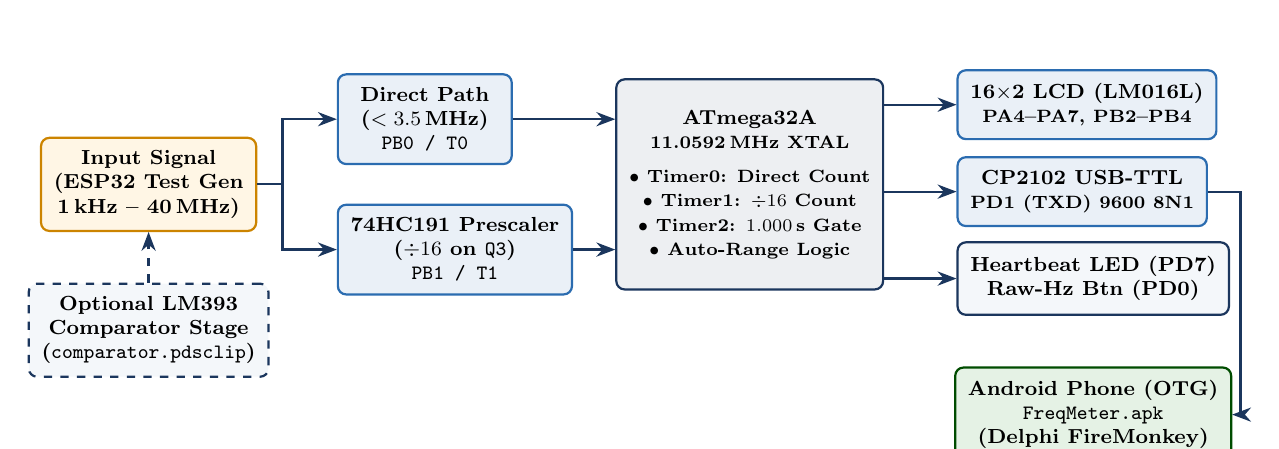
\begin{tikzpicture}[node distance=0.85cm and 0.95cm, scale=0.92, transform shape]
    % Input stage
    \node[block, fill=Orange!10, draw=Orange!80!black] (sig) {Input Signal\\(ESP32 Test Gen\\1\,kHz -- 40\,MHz)};
    \node[block, dashed, below=0.7cm of sig, minimum width=2.5cm] (comp) {Optional LM393\\Comparator Stage\\(\texttt{comparator.pdsclip})};

    % Split paths
    \node[hwblock, right=1.1cm of sig, yshift=0.9cm] (direct) {Direct Path\\($< 3.5\,\text{MHz}$)\\\texttt{PB0 / T0}};
    \node[hwblock, right=1.1cm of sig, yshift=-0.9cm] (presc) {74HC191 Prescaler\\($\div 16$ on \texttt{Q3})\\\texttt{PB1 / T1}};

    % MCU Core
    \node[block, anchor=west, minimum width=3.2cm, minimum height=2.9cm, fill=NavyPrimary!8] (mcu) at ($(direct.east)!0.5!(presc.east)+(1.0cm,0)$) {
        \textbf{ATmega32A}\\
        {\scriptsize 11.0592\,MHz XTAL}\\[4pt]
        {\scriptsize $\bullet$ Timer0: Direct Count}\\
        {\scriptsize $\bullet$ Timer1: $\div 16$ Count}\\
        {\scriptsize $\bullet$ Timer2: $1.000\,\text{s}$ Gate}\\
        {\scriptsize $\bullet$ Auto-Range Logic}
    };

    % Outputs
    \node[hwblock, right=1.0cm of mcu, yshift=1.1cm, minimum width=2.7cm] (lcd) {16$\times$2 LCD (LM016L)\\{\scriptsize PA4--PA7, PB2--PB4}};
    \node[hwblock, right=1.0cm of mcu, yshift=-0.1cm, minimum width=2.7cm] (uart) {CP2102 USB-TTL\\{\scriptsize PD1 (TXD) 9600 8N1}};
    \node[block, right=1.0cm of mcu, yshift=-1.3cm, minimum width=2.7cm] (io) {Heartbeat LED (PD7)\\Raw-Hz Btn (PD0)};

    % Android phone
    \node[block, fill=Green!10, draw=Green!60!black, below=0.7cm of io, minimum width=2.7cm] (app) {Android Phone (OTG)\\\texttt{FreqMeter.apk}\\(Delphi FireMonkey)};

    % Connections
    \draw[arrow] (sig.east) -- ++(0.35,0) |- (direct.west);
    \draw[arrow] (sig.east) -- ++(0.35,0) |- (presc.west);
    \draw[arrow, dashed] (comp.north) -- (sig.south);

    \draw[arrow] (direct.east) -- (mcu.west |- direct.east);
    \draw[arrow] (presc.east) -- (mcu.west |- presc.east);

    \draw[arrow] (mcu.east |- lcd.west) -- (lcd.west);
    \draw[arrow] (mcu.east |- uart.west) -- (uart.west);
    \draw[arrow] (mcu.east |- io.west) -- (io.west);
    \draw[arrow] (uart.east) -- ++(0.45,0) |- (app.east);
\end{tikzpicture}
\caption{End-to-end hardware and telemetry block diagram of the 40\,MHz frequency meter.}
\label{fig:block_diagram}
\end{figure}

\subsection{Dual-Range Measurement Theory and Overflow Extension}
According to the ATmega32 datasheet, external clock signals applied to pins \texttt{T0} (\texttt{PB0}) or \texttt{T1} (\texttt{PB1}) pass through an internal two-stage edge-synchronizer clocked by the CPU clock ($f_{\text{CPU}}$). To guarantee no missed edges, each logic level must be held for slightly longer than one CPU cycle, imposing a strict theoretical Nyquist-style ceiling of:
\begin{equation}
    f_{\text{ext,max}} = \frac{f_{\text{CPU}}}{2.5} = \frac{11.0592\,\text{MHz}}{2.5} \approx 4.42\,\text{MHz}.
\end{equation}
To measure signals up to $40\,\text{MHz}$ while preserving single-Hertz accuracy at lower frequencies, the incoming signal is routed simultaneously to two channels:
\begin{enumerate}[leftmargin=1.5em]
    \item \textbf{Direct Channel (Timer0 on \texttt{PB0/T0}):} Counts every rising edge directly. Because \texttt{TCNT0} is only 8 bits wide (overflowing every $256$ pulses), the overflow interrupt service routine (\texttt{timer0\_ovf\_isr}) increments a 32-bit volatile counter \texttt{Ovf0}, extending the counter to 40 bits:
    \begin{equation}
        f_{\text{direct}} = \left(\text{Ovf0} \times 256\right) + \text{TCNT0}.
    \end{equation}
    \item \textbf{Prescaled Channel (74HC191 $\div 16$ $\rightarrow$ Timer1 on \texttt{PB1/T1}):} The high-speed synchronous binary counter divides the incoming frequency by $16$ at output pin \texttt{Q3}. At $f_{\text{in}} = 40\,\text{MHz}$, the divided signal reaching \texttt{PB1/T1} is only $40\,\text{MHz} / 16 = 2.5\,\text{MHz}$, well below the $4.42\,\text{MHz}$ synchronization ceiling of the ATmega32. \texttt{Timer1} (16-bit) paired with its 32-bit overflow counter \texttt{Ovf1} reconstructs the full frequency as:
    \begin{equation}
        f_{\text{divided}} = \Big[\left(\text{Ovf1} \times 65{,}536\right) + \text{TCNT1}\Big] \times 16.
    \end{equation}
\end{enumerate}

\subsection{Exact 1.000\,s Gate Window Synthesis}
Choosing an \textbf{11.0592\,MHz} crystal solves two classical embedded design problems simultaneously:
\begin{itemize}[leftmargin=1.5em]
    \item \textbf{Zero-error UART Baud Rate:} For $9600\,\text{bps}$ in normal asynchronous mode ($\text{U2X}=0$),
    \begin{equation}
        \text{UBRR} = \frac{11{,}059{,}200}{16 \times 9600} - 1 = 72 - 1 = 71 \quad (\text{exact integer, } 0.00\% \text{ error}).
    \end{equation}
    \item \textbf{Exact 1.000000\,s Gate Window:} Clocking 8-bit \texttt{Timer2} through its $\div 1024$ prescaler yields an exact integer tick frequency:
    \begin{equation}
        f_{\text{T2}} = \frac{11{,}059{,}200\,\text{Hz}}{1024} = 10{,}800\,\text{ticks/s}.
    \end{equation}
    Since $10{,}800 = 42 \times 256 + 48$, preloading \texttt{TCNT2} with $256 - 48 = 208$ causes the first overflow after $48$ ticks and each subsequent overflow after $256$ ticks. Waiting for exactly $\text{Ovf2} = 43$ overflows produces:
    \begin{equation}
        N_{\text{ticks}} = (256 - 208) + 42 \times 256 = 48 + 10{,}752 = 10{,}800\text{ ticks} \equiv 1.000000\,\text{s}.
    \end{equation}
\end{itemize}

\subsection{Auto-Ranging Decision Logic}
At the end of each $1\,\text{s}$ gate, the firmware selects between $f_{\text{direct}}$ and $f_{\text{divided}}$ using a dual-condition threshold:
\begin{equation}
    f_{\text{final}} =
    \begin{cases}
        f_{\text{divided}}, & \text{if } f_{\text{divided}} > 3.5\,\text{MHz} \;\;\text{OR}\;\; f_{\text{divided}} > f_{\text{direct}} + 1000\,\text{Hz}, \\
        f_{\text{direct}}, & \text{otherwise.}
    \end{cases}
\end{equation}
The first guard ($> 3.5\,\text{MHz}$) switches cleanly to the prescaled channel with generous margin below the $4.42\,\text{MHz}$ MCU ceiling. The second guard ($f_{\text{divided}} > f_{\text{direct}} + 1000\,\text{Hz}$) acts as an intelligent \emph{aliasing fail-safe}: if an ultra-high-frequency signal causes \texttt{Timer0} to drop pulses or alias downward, $f_{\text{direct}}$ collapses while $f_{\text{divided}}$ remains accurate, forcing automatic selection of the prescaled channel.

% ============================================================================
%  SECTION 2: HARDWARE ARCHITECTURE & COMPONENTS
% ============================================================================
\section{Hardware Architecture and Component Specifications}

\subsection{Circuit Schematic}
Figure~\ref{fig:proteus_sim} displays the complete Proteus 8 schematic used for both VSM verification and physical breadboard wiring (shown here actively simulating a $20\,\text{MHz}$ input signal).

\begin{figure}[H]
    \centering
    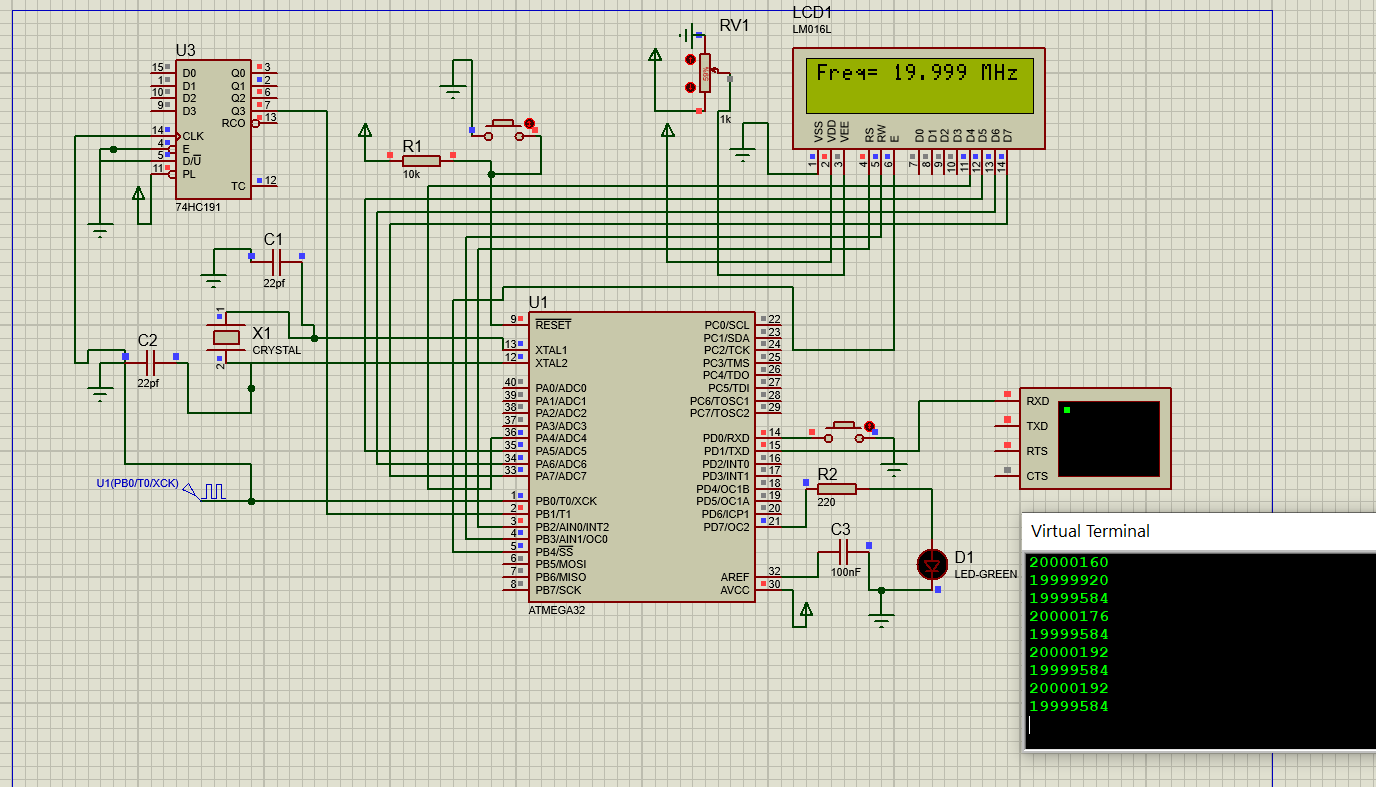
\includegraphics[width=\textwidth]{freq_sim.png}
    \caption{Complete Proteus 8 circuit schematic and live VSM simulation at $20\,\text{MHz}$, showing the ATmega32 (\texttt{U1}), 74HC191 $\div 16$ prescaler (\texttt{U3}), 11.0592\,MHz crystal (\texttt{X1}), $16\times 2$ LM016L LCD (\texttt{LCD1}), heartbeat LED (\texttt{D1}), mode/reset buttons, and Virtual Terminal UART output.}
    \label{fig:proteus_sim}
\end{figure}

\subsection{Detailed Hardware Component Breakdown}

\begin{enumerate}[leftmargin=1.5em]
    \item \textbf{Microcontroller --- Microchip ATmega32A (40-Pin DIP, \texttt{U1}):}
    An 8-bit CMOS AVR microcontroller with 32\,KB Flash, 2\,KB SRAM, three independent hardware timers (\texttt{Timer0}, \texttt{Timer1}, \texttt{Timer2}), and a hardware USART. All three timers are utilized simultaneously during each measurement window: \texttt{Timer0} as an 8-bit external counter, \texttt{Timer1} as a 16-bit external counter, and \texttt{Timer2} as the 1-second internal timebase.

    \item \textbf{Clock Oscillator --- 11.0592\,MHz Quartz Crystal (\texttt{X1}) + $2\times 22\,\text{pF}$ Capacitors (\texttt{C1, C2}):}
    Connected across \texttt{XTAL1} (pin~13) and \texttt{XTAL2} (pin~12) with 22\,pF load capacitors to ground. Provides high frequency stability ($\sim\pm 50\,\text{ppm}$), exact $10{,}800\,\text{ticks/s}$ gate timing, and $0.00\%$ UART baud error at $9600\,\text{bps}$.

    \item \textbf{High-Speed Prescaler --- SN74HC191N Synchronous 4-Bit Binary Counter (\texttt{U3}):}
    A high-speed silicon-gate CMOS 4-bit synchronous up/down counter operating up to $\sim 40\text{--}50\,\text{MHz}$ at $V_{CC} = 5\,\text{V}$. It is hard-wired as a free-running divide-by-16 prescaler:
    \begin{itemize}
        \item \texttt{CLK} (pin~14): Connected to the input signal (shared with \texttt{PB0/T0}).
        \item $\overline{\text{CE}}$ / Enable (pin~4) and \texttt{D/}$\overline{\text{U}}$ (pin~5): Tied to \texttt{GND} to permanently enable count-up mode.
        \item $\overline{\text{PL}}$ / Parallel Load (pin~11): Tied to $+5\,\text{V}$ (\texttt{VCC}) to disable parallel loading.
        \item \texttt{Q3} (pin~7): Most-significant bit output ($f_{\text{in}} / 16$), routed to ATmega32 \texttt{PB1/T1} (pin~2).
    \end{itemize}

    \item \textbf{Optional Analog Front-End --- LM393 Dual Comparator (\texttt{comparator.pdsclip}):}
    Saved as a modular Proteus design snippet for conditioning low-amplitude sinusoidal or AC signals into clean $0\text{--}5\,\text{V}$ CMOS square waves. Because our ESP32 test generator outputs clean digital square waves, the comparator stage can be bypassed during digital testing and inserted whenever measuring analog waveforms.

    \item \textbf{Local Display --- $16\times 2$ Alphanumeric LCD (\texttt{LM016L} / HD44780) + Contrast Potentiometer (\texttt{RV1}):}
    Interfaced in 4-bit parallel mode to conserve I/O pins: upper data nibble \texttt{D4--D7} connects to \texttt{PA4--PA7}, while control lines \texttt{RS}, \texttt{RW}, and \texttt{E} connect to \texttt{PB2}, \texttt{PB3}, and \texttt{PB4}. A rotary potentiometer (\texttt{RV1}, $1\,\text{k}\Omega\text{--}10\,\text{k}\Omega$) adjusts contrast on \texttt{VEE/V0}, and a series resistor limits LED backlight current on the real hardware module.

    \item \textbf{USB-to-UART Telemetry Bridge --- CP2102 Module + USB-OTG Adapter:}
    Converts the ATmega32's 5\,V TTL UART transmit line (\texttt{PD1/TXD}, pin~15) into a USB virtual COM interface connected directly to an Android smartphone via a Type-C USB-OTG adapter. In addition to carrying serial data, the CP2102's 5\,V bus can conveniently power the breadboard circuit from the phone during portable testing.

    \item \textbf{Reset, Mode Control, Decoupling, and Heartbeat Indicator:}
    \begin{itemize}
        \item \textbf{Reset Circuit:} $10\,\text{k}\Omega$ pull-up resistor (\texttt{R1}) on $\overline{\text{RESET}}$ (pin~9) paired with a momentary push-button to ground.
        \item \textbf{Raw-Hz Mode Button:} Momentary push-button between \texttt{PD0} (pin~14) and \texttt{GND}, using the ATmega32's internal pull-up resistor. Holding the button displays the unscaled 8-digit frequency in raw Hz on LCD line~2.
        \item \textbf{Heartbeat LED (\texttt{D1}):} Connected to \texttt{PD7} (pin~21) through a $220\,\Omega$ current-limiting resistor (\texttt{R2}); toggles state every $1\,\text{s}$ to provide immediate visual confirmation that the measurement loop is running.
        \item \textbf{Analog Reference Decoupling (\texttt{C3}):} $100\,\text{nF}$ ceramic capacitor on \texttt{AREF} (pin~32) with \texttt{AVCC} (pin~30) tied to $+5\,\text{V}$.
    \end{itemize}
\end{enumerate}

\subsection{Bill of Materials and Pinout Mapping}

\begin{table}[H]
\centering
\caption{Hardware Bill of Materials (BOM)}
\label{tab:bom}
\renewcommand{\arraystretch}{1.15}
\begin{tabularx}{\textwidth}{c l c X}
\toprule
\textbf{Ref} & \textbf{Component} & \textbf{Qty} & \textbf{Specification / Role} \\
\midrule
U1   & ATmega32A-PU (DIP-40)     & 1 & 8-bit AVR MCU, main controller \& counters \\
U3   & SN74HC191N (DIP-16)       & 1 & High-speed synchronous $\div 16$ prescaler (to 40\,MHz) \\
X1   & Quartz Crystal            & 1 & $11.0592\,\text{MHz}$ system clock \\
C1,C2& Ceramic Capacitors        & 2 & $22\,\text{pF}$ crystal load capacitors \\
C3   & Ceramic Capacitor         & 1 & $100\,\text{nF}$ decoupling capacitor (\texttt{AREF}) \\
LCD1 & $16\times 2$ HD44780 LCD  & 1 & Blue-backlight alphanumeric display (4-bit mode) \\
RV1  & Potentiometer             & 1 & $1\,\text{k}\Omega\text{--}10\,\text{k}\Omega$ LCD contrast adjustment \\
R1   & Resistor                  & 1 & $10\,\text{k}\Omega$ $\overline{\text{RESET}}$ pull-up \\
R2   & Resistor                  & 1 & $220\,\Omega$ heartbeat LED current limiter \\
D1   & LED (Green/Red)           & 1 & $1\,\text{Hz}$ measurement heartbeat indicator \\
SW1,2& Tactile Push-Buttons      & 2 & Hardware Reset + Raw-Hz display toggle (\texttt{PD0}) \\
---  & CP2102 USB-to-TTL Module  & 1 & UART-to-USB bridge for Android telemetry \\
---  & USB-OTG Adapter           & 1 & Type-C OTG adapter connecting CP2102 to phone \\
---  & ESP32 DevKit              & 1 & Programmable reference signal generator (testbench) \\
---  & Breadboards \& Jumpers    & 2 & 830-point interlocking solderless breadboards \\
\bottomrule
\end{tabularx}
\end{table}

\begin{table}[H]
\centering
\caption{ATmega32A Pin Assignment Map}
\label{tab:pinout}
\renewcommand{\arraystretch}{1.15}
\begin{tabularx}{\textwidth}{>{\ttfamily}l c l X}
\toprule
\textbf{MCU Pin} & \textbf{DIP Pin} & \textbf{Direction} & \textbf{Connected Peripheral / Function} \\
\midrule
PA4 -- PA7 & 36 -- 33 & Output & LCD1 Data Bus \texttt{D4 -- D7} (4-bit mode) \\
PB0 / T0   & 1        & Input  & Direct frequency input (Timer0 external clock, rising edge) \\
PB1 / T1   & 2        & Input  & 74HC191 \texttt{Q3} ($\div 16$ output, Timer1 external clock) \\
PB2        & 3        & Output & LCD1 \texttt{RS} (Register Select) \\
PB3        & 4        & Output & LCD1 \texttt{RW} (Read/Write, held LOW for write) \\
PB4        & 5        & Output & LCD1 \texttt{E} (Enable pulse) \\
PD0 / RXD  & 14       & Input  & Raw-Hz display mode push-button (internal pull-up, active LOW) \\
PD1 / TXD  & 15       & Output & UART TX ($9600\,\text{bps}$, 8N1) $\rightarrow$ CP2102 \texttt{RXD} \\
PD7        & 21       & Output & Heartbeat LED (\texttt{D1} via $220\,\Omega$ \texttt{R2}) \\
RESET      & 9        & Input  & $10\,\text{k}\Omega$ pull-up to $+5\,\text{V}$ + Reset button to GND \\
XTAL1/XTAL2& 13, 12   & Clock  & $11.0592\,\text{MHz}$ crystal + $2\times 22\,\text{pF}$ to GND \\
VCC, AVCC  & 10, 30   & Power  & $+5\,\text{V}$ rail (with $100\,\text{nF}$ on \texttt{AREF}, pin~32) \\
GND        & 11, 31   & Power  & Common ground shared with 74HC191, LCD, CP2102, and ESP32 \\
\bottomrule
\end{tabularx}
\end{table}

\subsection{Physical Breadboard Prototype}
Figure~\ref{fig:real_off} shows the completed breadboard prototype prior to power-up, highlighting the clean physical layout of the ATmega32A, crystal oscillator, SN74HC191N prescaler, $16\times 2$ LCD with contrast potentiometer, tactile buttons, heartbeat LED, and CP2102 USB-to-TTL module on the right edge.

\begin{figure}[H]
    \centering
    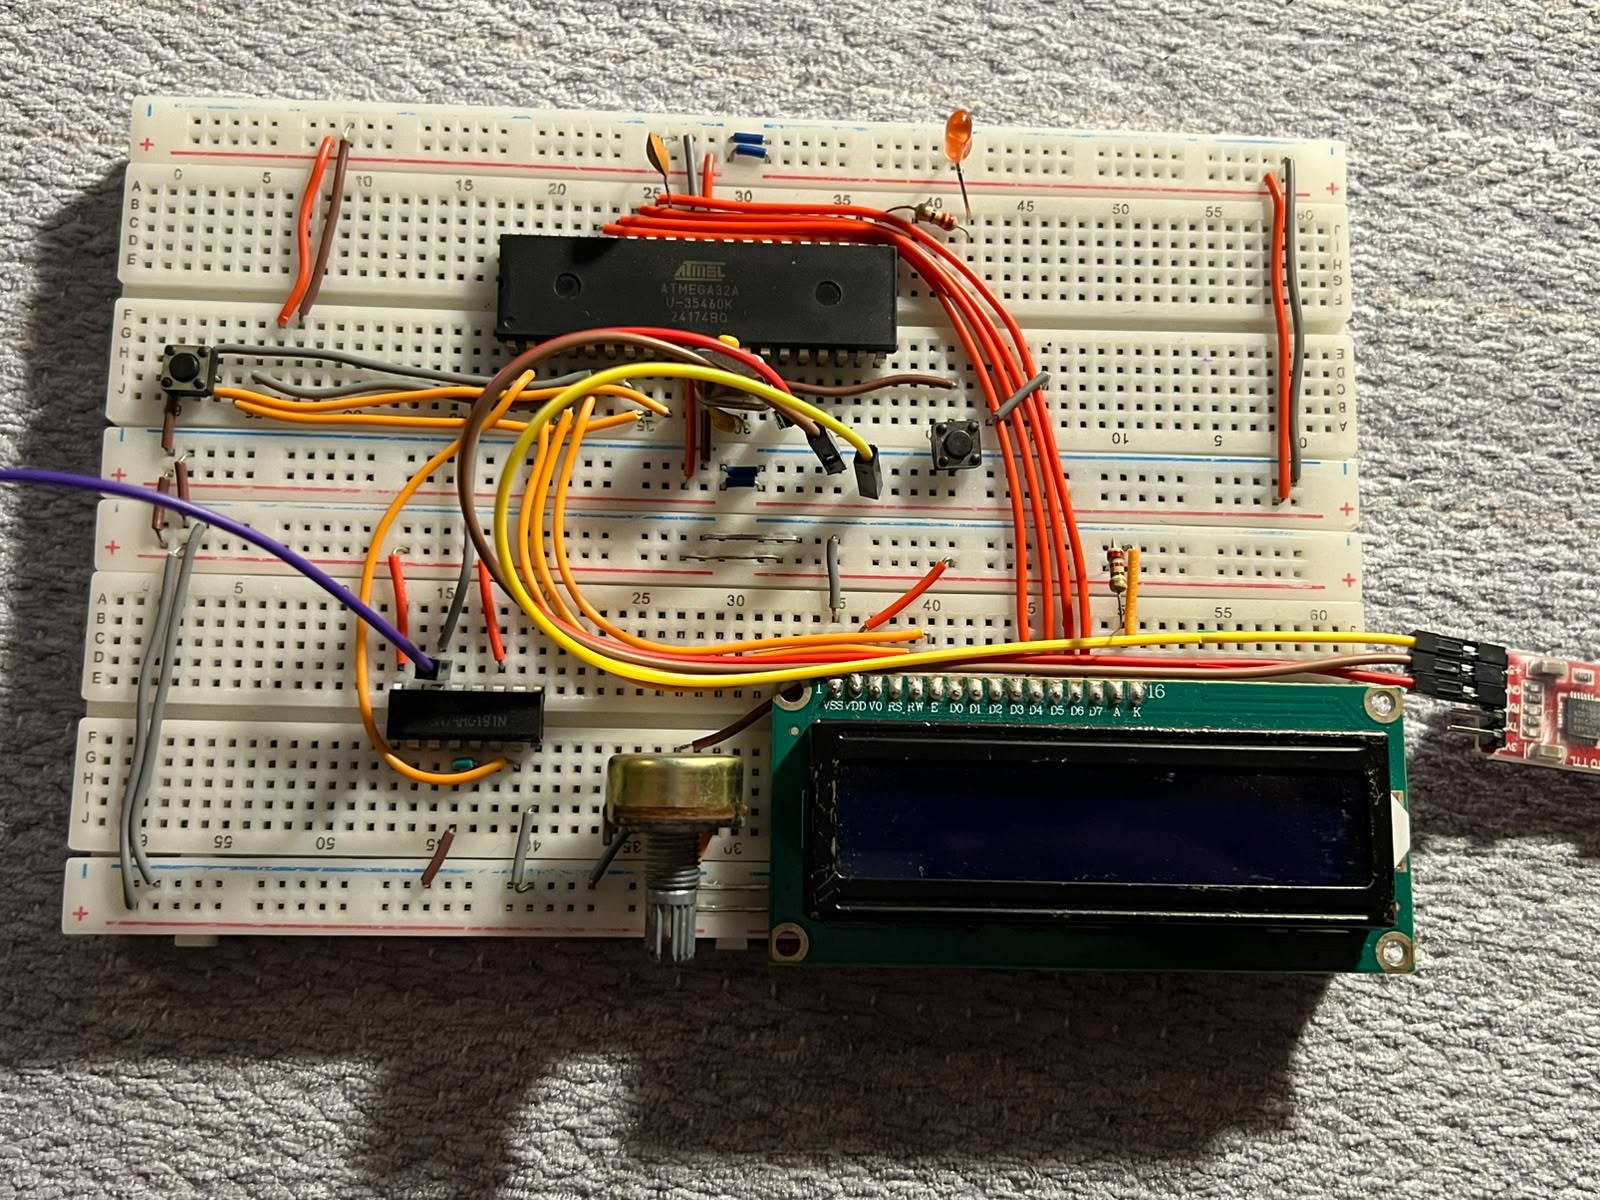
\includegraphics[width=0.9\textwidth]{real_circuit_off.jpeg}
    \caption{Assembled physical breadboard prototype (powered off) showing the ATmega32A (top center), 11.0592\,MHz crystal, SN74HC191N $\div 16$ prescaler (bottom left), $16\times 2$ LCD and contrast potentiometer (bottom right), tactile reset/mode switches, heartbeat LED (top), and CP2102 USB-to-TTL serial bridge (far right).}
    \label{fig:real_off}
\end{figure}

% ============================================================================
%  SECTION 3: SOURCE CODE REPOSITORY & HYPERLINKS
% ============================================================================
\section{Project Repository and Source Code Links}

All project artifacts---Proteus simulation files, CodeVisionAVR firmware, reusable AVR driver libraries, Embarcadero Delphi Android source code, the ESP32 pulse-generator sketch, and the signed Android APK---are hosted in our public GitHub repository at \href{\githubrepo}{\expandafter\printurl\expandafter{\githubrepo}}. Table~\ref{tab:links} provides direct clickable links to every file.

\begin{table}[H]
\centering\small
\caption{Source Code, Simulation, and Deliverable Hyperlinks}
\label{tab:links}
\renewcommand{\arraystretch}{1.22}
\begin{tabularx}{\textwidth}{l l X}
\toprule
\textbf{Category} & \textbf{File / Folder Link} & \textbf{Responsibility} \\
\midrule
Repository & \href{\githubrepo}{\texttt{m7mdelsayegh/frequency\_meter}} & Complete project repository \& documentation \\
\midrule
\multirow{2}{*}{Proteus 8}
    & \ghblob{1_Proteus_Simulation/freqmeter_c.pdsprj}{freqmeter\_c.pdsprj} & Main Proteus 8 schematic \& VSM simulation \\
    & \ghblob{1_Proteus_Simulation/comparator.pdsclip}{comparator.pdsclip} & Optional LM393 analog comparator design snippet \\
\midrule
\multirow{4}{*}{Firmware}
    & \ghblob{2_CodeVisionAVR_Firmware/main.c}{main.c} & Complete bare-metal ATmega32A firmware (timers, LCD, UART) \\
    & \ghblob{2_CodeVisionAVR_Firmware/freq_m.prj}{freq\_m.prj} & CodeVisionAVR project configuration ($11.0592\,\text{MHz}$) \\
    & \ghblob{2_CodeVisionAVR_Firmware/Debug/Exe/freq_m.hex}{freq\_m.hex} & Pre-compiled Intel HEX firmware for flashing / Proteus \\
    & \ghtree{2_CodeVisionAVR_Firmware/Driver_Libraries}{Driver\_Libraries/} & Reusable modular AVR drivers (DIO, LCD, TIMER, GIE) \\
\midrule
\multirow{5}{*}{Android App}
    & \ghblob{3_Delphi_Android_App/freq_m.dproj}{freq\_m.dproj} & Embarcadero RAD Studio / Delphi 12 Android 64-bit project \\
    & \ghblob{3_Delphi_Android_App/freq_meter.pas}{freq\_meter.pas} & Main UI logic, USB permission, background reader, parser \\
    & \ghblob{3_Delphi_Android_App/freq_meter.fmx}{freq\_meter.fmx} & FireMonkey visual form layout (Label, Button, Timer) \\
    & \ghblob{3_Delphi_Android_App/UsbSerialJNI.pas}{UsbSerialJNI.pas} & Delphi-to-Java JNI wrapper for Android USB \& Serial APIs \\
    & \ghblob{3_Delphi_Android_App/usb-serial.jar}{usb-serial.jar} & \texttt{usb-serial-for-android} Java library (CP21xx/CH34x/FTDI) \\
\midrule
Deliverable & \ghblob{4_Android_APK/FreqMeter.apk}{FreqMeter.apk} & Ready-to-install signed ARM64 Android APK \\
\midrule
Testbench & \ghblob{5_ESP32_Signal_Generator/esp32_freq_gen.ino}{esp32\_freq\_gen.ino} & ESP32 10-channel simultaneous square-wave generator ($1\,\text{kHz}$--$40\,\text{MHz}$) \\
\bottomrule
\end{tabularx}
\end{table}

% ============================================================================
%  SECTION 4: EMBEDDED FIRMWARE WORKFLOW (CODEVISIONAVR)
% ============================================================================
\section{Embedded Firmware Workflow (CodeVisionAVR --- ATmega32A)}

\subsection{Bare-Metal Architecture}
The production firmware resides in a single self-contained source file, \ghblob{2_CodeVisionAVR_Firmware/main.c}{main.c}, compiled by CodeVisionAVR v3.14 for the ATmega32 at $11.0592\,\text{MHz}$ (occupying only $2{,}136\,\text{bytes}$ of Flash, or $6.5\%$, and $100\,\text{bytes}$ of SRAM, or $4.9\%$). Rather than relying on heavy vendor HAL abstractions, all peripheral registers (\texttt{SREG}, \texttt{TCCR0/1/2}, \texttt{TCNT0/1/2}, \texttt{TIMSK}, \texttt{TIFR}, \texttt{UDR}, \texttt{UCSRA/B/C}, \texttt{UBRRH/L}, \texttt{PORTA/B/D}, \texttt{DDRA/B/D}) are accessed via direct \texttt{volatile u8*} memory-mapped macros. This minimizes interrupt latency---critical when \texttt{Timer0} overflows up to $13{,}671$ times per second at $3.5\,\text{MHz}$.

\subsection{Measurement Loop Flowchart}
Figure~\ref{fig:fw_flowchart} illustrates the deterministic 14-step execution flow performed every second inside \texttt{main()}.

\begin{figure}[H]
\centering
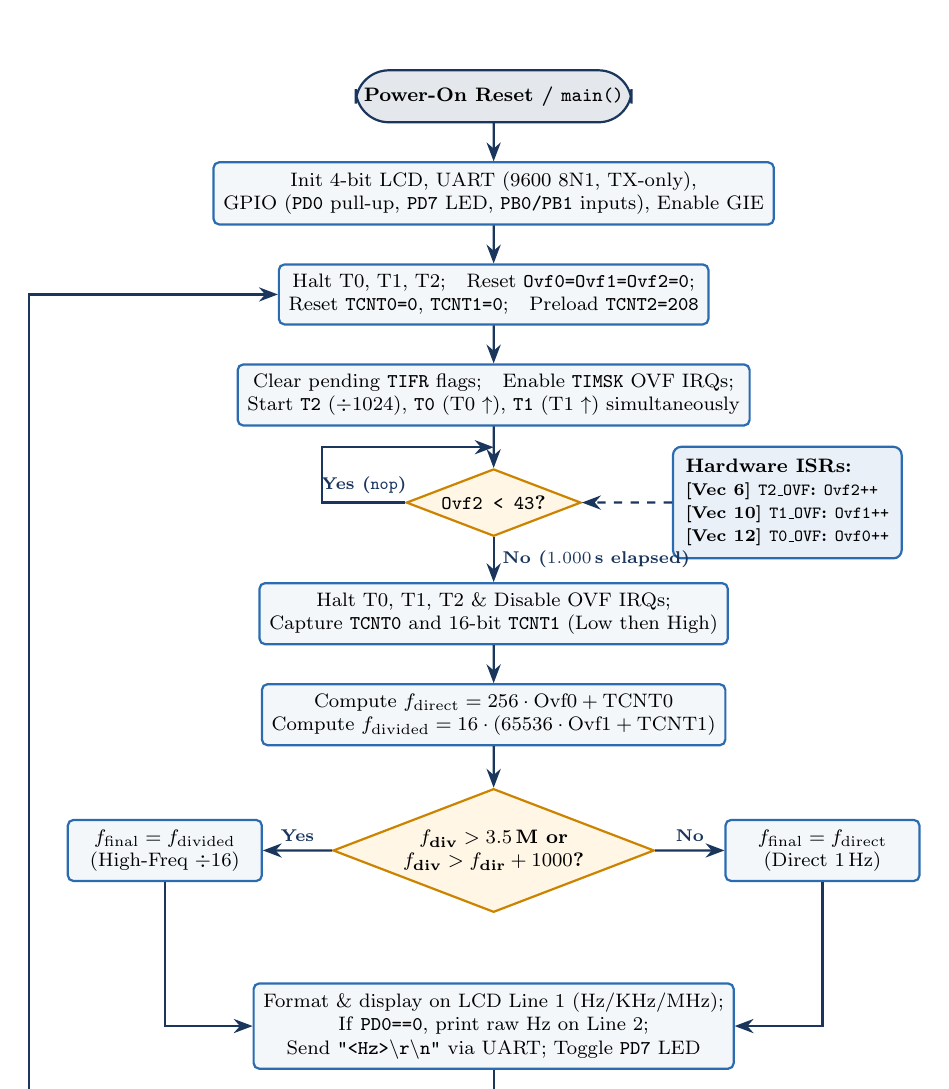
\begin{tikzpicture}[node distance=0.55cm and 0.9cm, scale=0.88, transform shape]
    \node[startstop] (start) {Power-On Reset / \texttt{main()}};
    \node[process, below=of start] (init) {Init 4-bit LCD, UART (9600 8N1, TX-only),\\GPIO (\texttt{PD0} pull-up, \texttt{PD7} LED, \texttt{PB0/PB1} inputs), Enable GIE};
    \node[process, below=of init] (prep) {Halt T0, T1, T2;\quad Reset \texttt{Ovf0=Ovf1=Ovf2=0};\\Reset \texttt{TCNT0=0}, \texttt{TCNT1=0};\quad Preload \texttt{TCNT2=208}};
    \node[process, below=of prep] (start_t) {Clear pending \texttt{TIFR} flags;\quad Enable \texttt{TIMSK} OVF IRQs;\\Start \texttt{T2} ($\div 1024$), \texttt{T0} (T0 $\uparrow$), \texttt{T1} (T1 $\uparrow$) simultaneously};
    \node[decision, below=0.6cm of start_t] (gate) {\texttt{Ovf2 < 43}?};
    \node[process, below=0.65cm of gate] (stop_t) {Halt T0, T1, T2 \& Disable OVF IRQs;\\Capture \texttt{TCNT0} and 16-bit \texttt{TCNT1} (Low then High)};
    \node[process, below=of stop_t] (calc) {Compute $f_{\text{direct}} = 256\cdot\text{Ovf0} + \text{TCNT0}$\\Compute $f_{\text{divided}} = 16\cdot(65536\cdot\text{Ovf1} + \text{TCNT1})$};
    \node[decision, below=0.6cm of calc] (sel) {$f_{\text{div}} > 3.5\,\text{M}$ or\\$f_{\text{div}} > f_{\text{dir}} + 1000$?};
    \node[process, left=1.0cm of sel, minimum width=2.8cm] (use_div) {$f_{\text{final}} = f_{\text{divided}}$\\(High-Freq $\div 16$)};
    \node[process, right=1.0cm of sel, minimum width=2.8cm] (use_dir) {$f_{\text{final}} = f_{\text{direct}}$\\(Direct $1\,\text{Hz}$)};
    \node[process, below=1.0cm of sel] (out) {Format \& display on LCD Line~1 (\text{Hz}/\text{KHz}/\text{MHz});\\If \texttt{PD0==0}, print raw Hz on Line~2;\\Send \texttt{"<Hz>\textbackslash r\textbackslash n"} via UART; Toggle \texttt{PD7} LED};

    % Side ISR box
    \node[hwblock, right=1.3cm of gate, minimum width=3.3cm, align=left] (isrs) {
        \textbf{Hardware ISRs:}\\
        {\scriptsize [Vec 6] \texttt{T2\_OVF}: \texttt{Ovf2++}}\\
        {\scriptsize [Vec 10] \texttt{T1\_OVF}: \texttt{Ovf1++}}\\
        {\scriptsize [Vec 12] \texttt{T0\_OVF}: \texttt{Ovf0++}}
    };

    % Arrows
    \draw[arrow] (start) -- (init);
    \draw[arrow] (init) -- (prep);
    \draw[arrow] (prep) -- (start_t);
    \draw[arrow] (start_t) -- (gate);
    \draw[arrow] (gate.west) -- ++(-1.2,0) node[above, pos=0.5, font=\scriptsize\bfseries]{Yes (\texttt{nop})} |- ($(start_t.south)!0.5!(gate.north)$);
    \draw[arrow] (gate.south) -- node[right, font=\scriptsize\bfseries]{No ($1.000\,\text{s}$ elapsed)} (stop_t.north);
    \draw[arrow, dashed] (isrs.west) -- (gate.east);
    \draw[arrow] (stop_t) -- (calc);
    \draw[arrow] (calc) -- (sel);
    \draw[arrow] (sel.west) -- node[above, font=\scriptsize\bfseries]{Yes} (use_div.east);
    \draw[arrow] (sel.east) -- node[above, font=\scriptsize\bfseries]{No} (use_dir.west);
    \draw[arrow] (use_div.south) |- (out.west);
    \draw[arrow] (use_dir.south) |- (out.east);
    \coordinate (loopback) at ($(use_div.west)+(-0.55cm,0)$);
    \draw[arrow] (out.south) -- ++(0,-0.45) -| (loopback) |- (prep.west);
\end{tikzpicture}
\caption{Execution workflow of the ATmega32A bare-metal firmware (\texttt{main.c}).}
\label{fig:fw_flowchart}
\end{figure}

\subsection{Detailed Module Workflows in \texttt{main.c}}

\subsubsection{Interrupt Service Routines (ISRs)}
Three minimal single-instruction ISRs use CodeVisionAVR's ATmega32 vector indices (1-based: vector~6 for \texttt{TIMER2\_OVF}, vector~10 for \texttt{TIMER1\_OVF}, and vector~12 for \texttt{TIMER0\_OVF}). Keeping each ISR to a single \texttt{volatile u32} increment prevents ISR stacking starvation even when counting multi-megahertz signals on \texttt{Timer0}.

\subsubsection{Hardware-Synced Capture and Atomic 16-Bit Read}
Before starting the gate, all pending overflow flags in \texttt{TIFR} (\texttt{TOV0}, \texttt{TOV1}, \texttt{TOV2}) are cleared by writing logic~\texttt{1} to bits~0, 2, and~6. Immediately after \texttt{Ovf2} reaches $43$, all three timers are halted (\texttt{TCCR0 = TCCR1B = TCCR2 = 0x00}) and overflow interrupts are masked. Per the ATmega32 16-bit register access rule, \texttt{TCNT1L} is always read \emph{before} \texttt{TCNT1H} so the hardware temporary buffer (\texttt{TEMP}) latches the high byte atomically:

\begin{lstlisting}[language=C, caption={Gate timing, simultaneous capture, and auto-ranging logic in \texttt{main.c}.}, label={lst:main_gate}]
/* Preload Timer2 for exact 1.000s @ 11.0592 MHz (43*256 - 208 = 10,800 ticks) */
TCNT0_register = 0;  TCNT1H_register = 0;  TCNT1L_register = 0;
TCNT2_register = 208;
TIFR_register  = (1 << 0) | (1 << 2) | (1 << 6);  /* Clear TOV0, TOV1, TOV2 */
TIMSK_register |= (1 << 0) | (1 << 2) | (1 << 6); /* Enable OVF interrupts  */

/* Start Timer2 (clk/1024), Timer0 (T0 rising), Timer1 (T1 rising) */
TCCR2_register = 0x07;  TCCR0_register = 0x07;  TCCR1B_register = 0x07;

while (Ovf2 < 43) { #asm("nop") }                 /* Exact 1.000s gate      */

/* Halt counters immediately and capture registers */
TCCR0_register = 0x00;  TCCR1B_register = 0x00;  TCCR2_register = 0x00;
TIMSK_register &= ~((1 << 0) | (1 << 2) | (1 << 6));

tcnt0_val = TCNT0_register;
low_b     = TCNT1L_register;                      /* Read LOW byte first    */
high_b    = TCNT1H_register;                      /* Then latched HIGH byte */
tcnt1_val = ((u16)high_b << 8) | low_b;

freq_direct  = (Ovf0 * 256UL) + tcnt0_val;
freq_divided = ((Ovf1 * 65536UL) + tcnt1_val) * 16UL;

/* Dual-condition auto-ranging with aliasing failover */
if (freq_divided > 3500000UL || (freq_divided > freq_direct + 1000UL))
    final_freq = freq_divided;
else
    final_freq = freq_direct;
\end{lstlisting}

\subsubsection{TX-Only UART Driver (\texttt{UART\_Init}, \texttt{UART\_Send\_Freq})}
A subtle hardware optimization appears in \texttt{UART\_Init()}: setting \texttt{UCSRB = 0x08} enables \emph{only} the hardware transmitter (\texttt{TXEN = 1}) while keeping the receiver disabled (\texttt{RXEN = 0}). This deliberately leaves pin \texttt{PD0/RXD} free as a standard digital GPIO input with internal pull-up for the Raw-Hz push-button! \texttt{UART\_Send\_Freq()} converts the unsigned 32-bit frequency into decimal ASCII digits without linking \texttt{sprintf()} (saving Flash and stack) and appends \texttt{\textbackslash r\textbackslash n} (\texttt{CRLF}), matching the line-delimited protocol expected by the Delphi Android application.

\subsubsection{4-Bit LCD Driver and Auto-Scaling Display}
\texttt{LCD\_Init()} initializes the HD44780 controller in 4-bit, 2-line, display-on mode (\texttt{0x02}, \texttt{0x28}, \texttt{0x0C}, \texttt{0x01}, \texttt{0x06}) using \texttt{PA4--PA7} and \texttt{PB2--PB4}. Three dedicated formatters---\texttt{MHz()}, \texttt{KHz()}, and \texttt{Hz()}---select the appropriate engineering prefix on line~1, while \texttt{display()} prints the full 8-digit integer frequency in Hz on line~2 whenever \texttt{PD0} is pressed LOW.

\subsection{Reusable Layered Driver Libraries (\texttt{Driver\_Libraries/})}
Alongside the self-contained \texttt{main.c}, the repository preserves a modular MCAL/HAL driver stack in \ghtree{2_CodeVisionAVR_Firmware/Driver_Libraries}{Driver\_Libraries/} designed for reusable AVR embedded projects:
\begin{itemize}[leftmargin=1.5em]
    \item \texttt{STD\_TYPES.h} \& \texttt{BIT\_MATH.h}: Portable fixed-width typedefs (\texttt{u8}, \texttt{u16}, \texttt{u32}, \texttt{s8}--\texttt{s32}) and bit-manipulation macros (\texttt{Set\_Bit}, \texttt{Clr\_Bit}, \texttt{Tog\_Bit}, \texttt{Get\_Bit}).
    \item \texttt{DIO\_register.h / \_interface.h / \_program.c}: Port and pin direction, read, write, and toggle abstractions across \texttt{PORTA--PORTD}.
    \item \texttt{LCD\_config.h / \_interface.h / \_program.c}: Configurable 4-bit HD44780 LCD driver built on top of the DIO layer.
    \item \texttt{TIMER\_register.h / \_config.h / \_interface.h / \_program.c}: Callback-driven Timer0 and Timer1 drivers with CodeVisionAVR interrupt vectors and atomic 16-bit \texttt{TCNT1} helpers.
    \item \texttt{GLOBAL\_INTERRUPT\_register.h / \_interface.h / \_program.c}: Global interrupt enable/disable wrapper over the \texttt{SREG} I-bit.
\end{itemize}

% ============================================================================
%  SECTION 5: ANDROID APPLICATION WORKFLOW (DELPHI / FIREMONKEY)
% ============================================================================
\section{Android Companion App Workflow (Embarcadero Delphi 12)}

\subsection{Cross-Layer JNI Architecture}
The mobile companion app is built with \textbf{Embarcadero RAD Studio / Delphi 12 (Studio 23.0)} using the FireMonkey (FMX) framework targeting \textbf{Android 64-bit (ARM64-v8a)}. Because Android does not expose raw USB-serial devices as Linux \texttt{/dev/ttyUSB*} nodes to unprivileged apps, the application communicates through Android's Java \texttt{android.hardware.usb} host API and the open-source \texttt{usb-serial-for-android} Java library (\ghblob{3_Delphi_Android_App/usb-serial.jar}{usb-serial.jar}), bridged into native Delphi ARM64 code via the Java Native Interface (JNI) in \ghblob{3_Delphi_Android_App/UsbSerialJNI.pas}{UsbSerialJNI.pas}. Figure~\ref{fig:android_stack} depicts this software stack.

\begin{figure}[H]
\centering
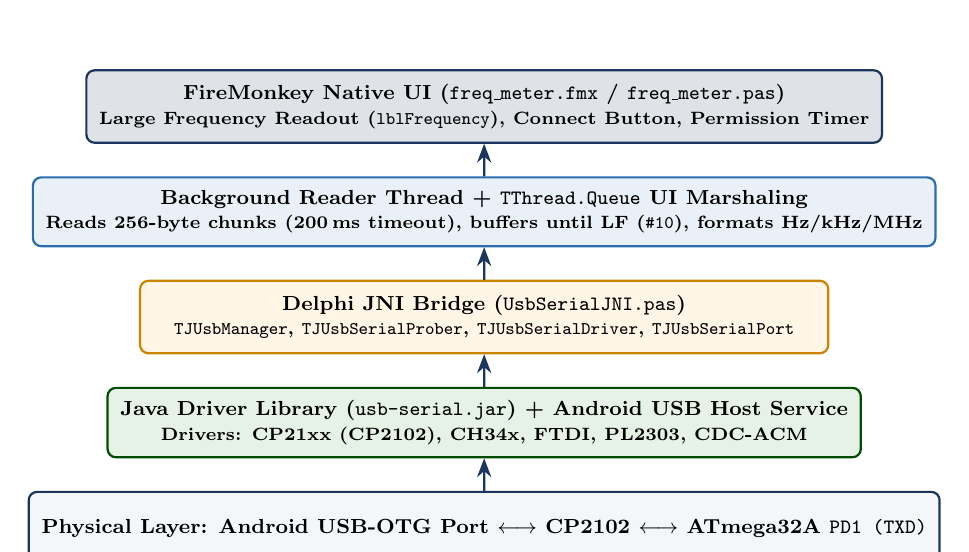
\begin{tikzpicture}[node distance=0.45cm, scale=0.92, transform shape]
    \node[block, minimum width=9.5cm, fill=NavyPrimary!14] (ui) {FireMonkey Native UI (\texttt{freq\_meter.fmx} / \texttt{freq\_meter.pas})\\{\scriptsize Large Frequency Readout (\texttt{lblFrequency}), Connect Button, Permission Timer}};
    \node[hwblock, below=of ui, minimum width=9.5cm] (thread) {Background Reader Thread + \texttt{TThread.Queue} UI Marshaling\\{\scriptsize Reads 256-byte chunks (200\,ms timeout), buffers until LF (\texttt{\#10}), formats Hz/kHz/MHz}};
    \node[block, below=of thread, minimum width=9.5cm, fill=Orange!10, draw=Orange!80!black] (jni) {Delphi JNI Bridge (\texttt{UsbSerialJNI.pas})\\{\scriptsize \texttt{TJUsbManager}, \texttt{TJUsbSerialProber}, \texttt{TJUsbSerialDriver}, \texttt{TJUsbSerialPort}}};
    \node[hwblock, below=of jni, minimum width=9.5cm, fill=Green!10, draw=Green!60!black] (jar) {Java Driver Library (\texttt{usb-serial.jar}) + Android USB Host Service\\{\scriptsize Drivers: CP21xx (CP2102), CH34x, FTDI, PL2303, CDC-ACM}};
    \node[block, below=of jar, minimum width=9.5cm, fill=SoftBg] (hw) {Physical Layer: Android USB-OTG Port $\longleftrightarrow$ CP2102 $\longleftrightarrow$ ATmega32A \texttt{PD1 (TXD)}};

    \draw[arrow] (hw) -- (jar);
    \draw[arrow] (jar) -- (jni);
    \draw[arrow] (jni) -- (thread);
    \draw[arrow] (thread) -- (ui);
\end{tikzpicture}
\caption{Layered architecture of the Embarcadero Delphi Android USB-OTG companion app.}
\label{fig:android_stack}
\end{figure}

\subsection{File-by-File Code Workflow}

\begin{enumerate}[leftmargin=1.5em]
    \item \textbf{Project Entry \& Build Files (\ghblob{3_Delphi_Android_App/freq_m.dpr}{freq\_m.dpr}, \ghblob{3_Delphi_Android_App/freq_m.dproj}{freq\_m.dproj}, \ghblob{3_Delphi_Android_App/AndroidManifest.template.xml}{AndroidManifest.template.xml}):}
    \texttt{freq\_m.dpr} initializes the FireMonkey runtime and creates \texttt{Form1}. \texttt{freq\_m.dproj} registers \texttt{usb-serial.jar} under Android~64-bit Java libraries so RAD Studio dexes and packages its classes into the APK's \texttt{classes.dex}. \texttt{AndroidManifest.template.xml} configures the native activity (\texttt{FMXNativeActivity}) and permissions.

    \item \textbf{JNI Wrapper (\ghblob{3_Delphi_Android_App/UsbSerialJNI.pas}{UsbSerialJNI.pas}):}
    Declares Delphi interface pairs (\texttt{J*Class} and \texttt{J*}) annotated with \texttt{[JavaSignature(...)]} and wrapped via \texttt{TJavaGenericImport<C,I>}. It exposes six Java classes/interfaces:
    \begin{itemize}
        \item \texttt{android/hardware/usb/UsbManager}: \texttt{hasPermission}, \texttt{requestPermission}, \texttt{openDevice}.
        \item \texttt{android/hardware/usb/UsbDevice} \& \texttt{UsbDeviceConnection}.
        \item \texttt{com/hoho/android/usbserial/driver/UsbSerialProber}: static \texttt{getDefaultProber} and \texttt{findAllDrivers}.
        \item \texttt{UsbSerialDriver} (\texttt{getDevice}, \texttt{getPorts}) and \texttt{UsbSerialPort} (\texttt{open}, \texttt{close}, \texttt{setParameters}, \texttt{read}, \texttt{write}).
    \end{itemize}

    \item \textbf{UI Layout (\ghblob{3_Delphi_Android_App/freq_meter.fmx}{freq\_meter.fmx}):}
    Defines a clean portrait mobile layout containing three components:
    \begin{itemize}
        \item \texttt{lblFrequency} (\texttt{TLabel}): Top-aligned, centered 42\,pt display initialized to \texttt{"--- Hz"}.
        \item \texttt{btnConnect} (\texttt{TButton}): Initiates USB device probing and serial connection.
        \item \texttt{tmrPermission} (\texttt{TTimer}): Disabled by default; polls every $500\,\text{ms}$ while waiting for the user to approve Android's USB permission dialog.
    \end{itemize}

    \item \textbf{Application Logic (\ghblob{3_Delphi_Android_App/freq_meter.pas}{freq\_meter.pas}):}
    Follows the runtime state machine illustrated in Figure~\ref{fig:app_flowchart}:
    \begin{itemize}
        \item \textbf{Device Discovery (\texttt{btnConnectClick}):} Retrieves the Android \texttt{"usb"} system service and calls \texttt{UsbSerialProber.getDefaultProber.findAllDrivers(FManager)}. If no USB-serial bridge is attached, displays \texttt{"No USB device"}.
        \item \textbf{Android 12+ Mutable Permission Request:} Checks \texttt{FManager.hasPermission(Dev)}. If ungranted, creates an explicit broadcast \texttt{PendingIntent} with \texttt{FLAG\_MUTABLE} (\texttt{\$02000000})---required on modern Android SDKs so the OS can populate the granted-permission extras---calls \texttt{requestPermission}, and activates \texttt{tmrPermission}.
        \item \textbf{Port Opening (\texttt{OpenPort}):} Opens the USB device connection, binds port~0, configures \textbf{9600 baud, 8 data bits, 1 stop bit, parity 0 (None)}, sets \texttt{"Waiting for data..."}, and launches \texttt{StartReading}.
        \item \textbf{Asynchronous Reading \& Line Parsing (\texttt{StartReading}, \texttt{PostChunk}, \texttt{HandleIncoming}):} Spawns an anonymous worker thread that blocks on \texttt{FPort.read(Buf, 200)} using a reusable 256-byte \texttt{TJavaArray<Byte>}. Received bytes are decoded as ASCII and marshaled to the main UI thread via \texttt{TThread.Queue}. \texttt{HandleIncoming} appends chunks to \texttt{RxBuffer}, splits complete lines on LF (\texttt{\#10}), parses them via \texttt{TryStrToInt64}, and updates \texttt{lblFrequency.Text} using \texttt{FormatFreq()} (auto-formatting as \texttt{Hz}, \texttt{kHz}, or \texttt{MHz} with 3 decimal places).
        \item \textbf{Graceful Shutdown (\texttt{FormDestroy}):} Clears \texttt{FReading := False} and closes \texttt{FPort} cleanly to release the USB interface.
    \end{itemize}
\end{enumerate}

\begin{figure}[H]
\centering
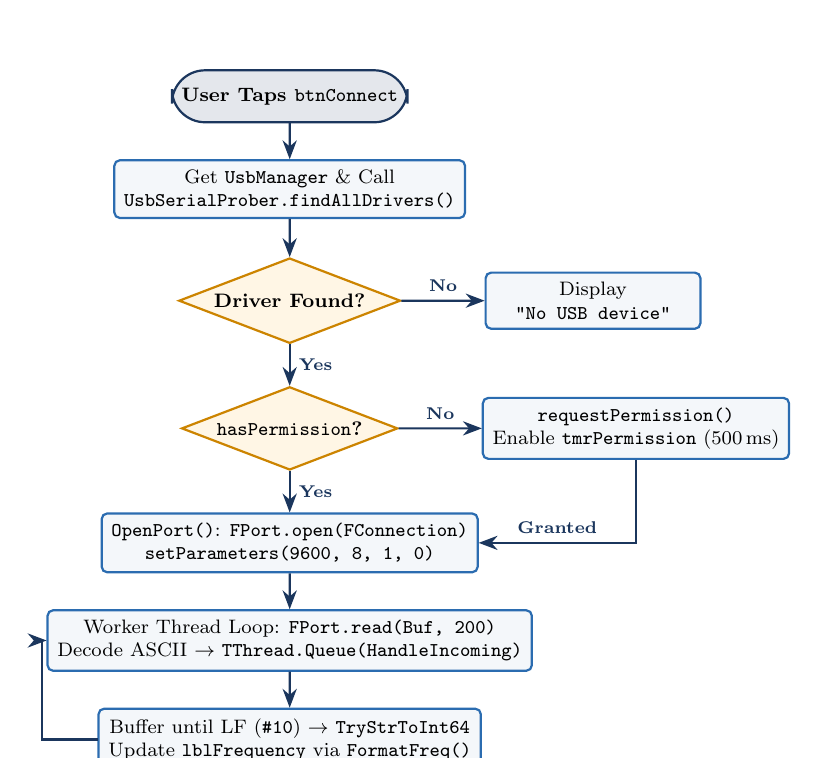
\begin{tikzpicture}[node distance=0.52cm and 1.1cm, scale=0.88, transform shape]
    \node[startstop] (tap) {User Taps \texttt{btnConnect}};
    \node[process, below=of tap] (probe) {Get \texttt{UsbManager} \& Call\\ \texttt{UsbSerialProber.findAllDrivers()}};
    \node[decision, below=0.55cm of probe] (found) {Driver Found?};
    \node[process, right=1.2cm of found, minimum width=3.1cm] (nodev) {Display\\\texttt{"No USB device"}};
    \node[decision, below=0.6cm of found] (perm) {\texttt{hasPermission}?};
    \node[process, right=1.2cm of perm, minimum width=3.4cm] (req) {\texttt{requestPermission()}\\Enable \texttt{tmrPermission} (500\,ms)};
    \node[process, below=0.6cm of perm] (open) {\texttt{OpenPort()}: \texttt{FPort.open(FConnection)}\\ \texttt{setParameters(9600, 8, 1, 0)}};
    \node[process, below=of open] (bg) {Worker Thread Loop: \texttt{FPort.read(Buf, 200)}\\Decode ASCII $\rightarrow$ \texttt{TThread.Queue(HandleIncoming)}};
    \node[process, below=of bg] (parse) {Buffer until LF (\texttt{\#10}) $\rightarrow$ \texttt{TryStrToInt64}\\Update \texttt{lblFrequency} via \texttt{FormatFreq()}};

    \draw[arrow] (tap) -- (probe);
    \draw[arrow] (probe) -- (found);
    \draw[arrow] (found.east) -- node[above, font=\scriptsize\bfseries]{No} (nodev.west);
    \draw[arrow] (found.south) -- node[right, font=\scriptsize\bfseries]{Yes} (perm.north);
    \draw[arrow] (perm.east) -- node[above, font=\scriptsize\bfseries]{No} (req.west);
    \draw[arrow] (req.south) |- node[near end, above, font=\scriptsize\bfseries]{Granted} (open.east);
    \draw[arrow] (perm.south) -- node[right, font=\scriptsize\bfseries]{Yes} (open.north);
    \draw[arrow] (open) -- (bg);
    \draw[arrow] (bg) -- (parse);
    \draw[arrow] (parse.west) -- ++(-0.8,0) |- (bg.west);
\end{tikzpicture}
\caption{Runtime connection, permission, and serial-streaming workflow of \texttt{freq\_meter.pas}.}
\label{fig:app_flowchart}
\end{figure}

\begin{lstlisting}[language=Pascal, caption={Line-delimited serial parsing and auto-unit formatting in \texttt{freq\_meter.pas}.}, label={lst:delphi_parse}]
function FormatFreq(Hz: Int64): string;
begin
  if Hz >= 1000000 then
    Result := Format('%.3f MHz', [Hz / 1e6], TFormatSettings.Invariant)
  else if Hz >= 1000 then
    Result := Format('%.3f kHz', [Hz / 1e3], TFormatSettings.Invariant)
  else
    Result := Format('%d Hz', [Hz]);
end;

procedure TForm1.HandleIncoming(const Chunk: string);
var
  P: Integer;
  Line: string;
  Freq: Int64;
begin
  RxBuffer := RxBuffer + Chunk;
  P := RxBuffer.IndexOf(#10);               // Split on LF sent by ATmega32
  while P >= 0 do
  begin
    Line := RxBuffer.Substring(0, P).Trim;  // Strip CR and whitespace
    RxBuffer := RxBuffer.Substring(P + 1);
    if TryStrToInt64(Line, Freq) then
      lblFrequency.Text := FormatFreq(Freq);
    P := RxBuffer.IndexOf(#10);
  end;
end;
\end{lstlisting}

% ============================================================================
%  SECTION 6: ESP32 MULTI-FREQUENCY PULSE GENERATOR (TESTBENCH)
% ============================================================================
\section{ESP32 Multi-Frequency Pulse Generator (Hardware Testbench)}
\label{sec:esp_gen}

\subsection{Architecture and Hardware PWM Principle}
To thoroughly test the frequency meter across its entire $1\,\text{kHz}$ to $40\,\text{MHz}$ operating range---including the exact $3.5\,\text{MHz}$ auto-switching threshold---without requiring a benchtop RF function generator, we programmed an \textbf{ESP32 DevKit} as a \textbf{10-channel simultaneous square-wave pulse generator} (\ghblob{5_ESP32_Signal_Generator/esp32_freq_gen.ino}{esp32\_freq\_gen.ino}).

The design leverages the ESP32's hardware \textbf{LEDC (LED Control) PWM peripheral}, which is clocked directly from the crystal-stabilized $80\,\text{MHz}$ APB bus:
\begin{itemize}[leftmargin=1.5em]
    \item \textbf{1-Bit Resolution for Maximum Frequency Ceiling:} For a given PWM bit resolution $R$, the maximum output frequency of an LEDC channel is bounded by:
    \begin{equation}
        f_{\text{LEDC,max}} = \frac{f_{\text{APB}}}{2^{R}}.
    \end{equation}
    Setting \texttt{pwmResolution = 1} ($R = 1$) minimizes the counter modulus to $2^{1} = 2$ steps per cycle, unlocking the absolute hardware maximum frequency of $80\,\text{MHz} / 2 = 40.000\,\text{MHz}$.
    \item \textbf{Exact 50\% Duty Cycle:} Writing a duty count of \texttt{1} via \texttt{ledcWrite(pin, 1)} sets the output HIGH for $1$ tick and LOW for $1$ tick out of every $2$-tick period, yielding a clean $50\%$ duty-cycle square wave on every channel.
    \item \textbf{Zero CPU Overhead:} Once \texttt{setup()} configures all ten LEDC channels, the hardware timers and GPIO matrix generate all square waves autonomously with zero software jitter; \texttt{loop()} remains completely empty.
    \item \textbf{Strategic Boundary Coverage:} Having dedicated pins at $3\,\text{MHz}$ (\texttt{GPIO 4}), $4\,\text{MHz}$ (\texttt{GPIO 16}), and $5\,\text{MHz}$ (\texttt{GPIO 17}) allows instant single-wire probing right below and right above the ATmega32A's $3.5\,\text{MHz}$ auto-range switchover and $4.42\,\text{MHz}$ native counter ceiling.
\end{itemize}

\subsection{ESP32 GPIO Pin-to-Frequency Output Map}
Table~\ref{tab:esp_pins} documents every GPIO pin configured by \texttt{esp32\_freq\_gen.ino}, its exact target frequency, signal period, duty cycle, and the corresponding ATmega32A measurement channel exercised during testing.

\begin{table}[H]
\centering\small
\caption{ESP32 Pulse Generator Pin-to-Frequency Mapping (\texttt{esp32\_freq\_gen.ino})}
\label{tab:esp_pins}
\renewcommand{\arraystretch}{1.18}
\begin{tabularx}{\textwidth}{>{\ttfamily\bfseries}c r c c X}
\toprule
\textbf{ESP32 Pin} & \textbf{Output Frequency} & \textbf{Period} & \textbf{Duty} & \textbf{Target Meter Channel / Test Purpose} \\
\midrule
GPIO 25 & $1\,\text{kHz}$   & $1.00\,\text{ms}$   & $50\%$ & Direct (\texttt{PB0/T0}) --- low-frequency accuracy \\
GPIO 26 & $10\,\text{kHz}$  & $100\,\mu\text{s}$  & $50\%$ & Direct (\texttt{PB0/T0}) --- audio/mid-range check \\
GPIO 27 & $100\,\text{kHz}$ & $10\,\mu\text{s}$   & $50\%$ & Direct (\texttt{PB0/T0}) --- high-kHz stability \\
GPIO 32 & $1\,\text{MHz}$   & $1.00\,\mu\text{s}$ & $50\%$ & Direct (\texttt{PB0/T0}) --- MHz formatting check \\
GPIO 4  & $3\,\text{MHz}$   & $333.3\,\text{ns}$  & $50\%$ & Direct (\texttt{PB0/T0}) --- just below $3.5\,\text{MHz}$ threshold \\
\midrule
GPIO 16 & $4\,\text{MHz}$   & $250.0\,\text{ns}$  & $50\%$ & Prescaled $\div 16$ (\texttt{PB1/T1}) --- triggers auto-switch ($>3.5\,\text{MHz}$) \\
GPIO 17 & $5\,\text{MHz}$   & $200.0\,\text{ns}$  & $50\%$ & Prescaled $\div 16$ (\texttt{PB1/T1}) --- above $4.42\,\text{MHz}$ MCU ceiling \\
GPIO 18 & $10\,\text{MHz}$  & $100.0\,\text{ns}$  & $50\%$ & Prescaled $\div 16$ (\texttt{PB1/T1}) --- $625\,\text{kHz}$ at \texttt{T1} \\
GPIO 14 & $30\,\text{MHz}$  & $33.3\,\text{ns}$   & $50\%$ & Prescaled $\div 16$ (\texttt{PB1/T1}) --- $1.875\,\text{MHz}$ at \texttt{T1} \\
GPIO 13 & $40\,\text{MHz}$  & $25.0\,\text{ns}$   & $50\%$ & Prescaled $\div 16$ (\texttt{PB1/T1}) --- $2.500\,\text{MHz}$ at \texttt{T1} (full-scale max) \\
\bottomrule
\end{tabularx}
\end{table}

\begin{infobox}[Hardware Testing Connection]
To test any frequency in Table~\ref{tab:esp_pins}, connect a single short jumper wire from the desired ESP32 GPIO pin to the frequency meter input node (shared by ATmega32A \texttt{PB0/T0} and 74HC191 \texttt{CLK}), and tie \texttt{GND} of the ESP32 to the breadboard ground rail. Note that on the ESP32, the 16 LEDC channels share 8 hardware timers; the Arduino-ESP32 v3.x \texttt{ledcAttach()} API automatically allocates timers and prints \texttt{: OK} or \texttt{: ERROR} per pin over the $115200\,\text{bps}$ Serial Monitor for instant diagnostic confirmation.
\end{infobox}

\subsection{Code Workflow and Source Listing}
The firmware workflow of \ghblob{5_ESP32_Signal_Generator/esp32_freq_gen.ino}{esp32\_freq\_gen.ino} executes strictly during initialization:
\begin{enumerate}[leftmargin=1.5em]
    \item Initializes USB serial logging at $115200\,\text{bps}$ and prints the startup banner.
    \item Iterates across the two parallel lookup tables \texttt{outputPins[10]} and \texttt{frequencies[10]}.
    \item Calls \texttt{ledcAttach(outputPins[i], frequencies[i], 1)} (Arduino-ESP32 Core v3.x unified LEDC API) to bind each GPIO pin to a hardware PWM timer at 1-bit resolution.
    \item On success, writes duty cycle \texttt{1} via \texttt{ledcWrite()} for a $50\%$ square wave and logs the human-readable unit (\texttt{MHz}, \texttt{kHz}, or \texttt{Hz}) with \texttt{: OK}; otherwise prints \texttt{: ERROR}.
    \item Exits \texttt{setup()} into an empty \texttt{loop()} while the LEDC hardware sustains all waveforms continuously.
\end{enumerate}

\begin{lstlisting}[language=C++, caption={Complete ESP32 10-channel square-wave pulse generator (\texttt{esp32\_freq\_gen.ino}).}, label={lst:esp32_gen}]
const int NUM_CHANNELS = 10;

const int outputPins[NUM_CHANNELS] = {
  13, 14, 25, 26, 27, 32, 4, 16, 17, 18
};

const uint32_t frequencies[NUM_CHANNELS] = {
  40000000, // GPIO 13 -> 40 MHz
  30000000, // GPIO 14 -> 30 MHz
  1000,     // GPIO 25 -> 1 kHz
  10000,    // GPIO 26 -> 10 kHz
  100000,   // GPIO 27 -> 100 kHz
  1000000,  // GPIO 32 -> 1 MHz
  3000000,  // GPIO 4  -> 3 MHz
  4000000,  // GPIO 16 -> 4 MHz
  5000000,  // GPIO 17 -> 5 MHz
  10000000  // GPIO 18 -> 10 MHz
};

// 1-bit resolution allows 50% duty cycle up to 40 MHz max
const uint8_t pwmResolution = 1;

void setup() {
  Serial.begin(115200);
  Serial.println();
  Serial.println("ESP32 Multi-Frequency Square Wave Generator");
  Serial.println("-------------------------------------------");

  for (int i = 0; i < NUM_CHANNELS; i++) {
    bool configured = ledcAttach(outputPins[i], frequencies[i], pwmResolution);

    if (configured) {
      ledcWrite(outputPins[i], 1); // 50% duty cycle (1 out of 2^1)

      Serial.print("GPIO ");
      if (outputPins[i] < 10) Serial.print(" ");
      Serial.print(outputPins[i]);
      Serial.print(" -> ");

      if (frequencies[i] >= 1000000) {
        Serial.print(frequencies[i] / 1000000); Serial.print(" MHz");
      } else if (frequencies[i] >= 1000) {
        Serial.print(frequencies[i] / 1000);    Serial.print(" kHz");
      } else {
        Serial.print(frequencies[i]);           Serial.print(" Hz");
      }
      Serial.println(" : OK");
    } else {
      Serial.print("GPIO "); Serial.print(outputPins[i]);
      Serial.println(" : ERROR");
    }
  }
  Serial.println("-------------------------------------------");
  Serial.println("All 10 PWM outputs configured successfully.");
}

void loop() {
  // Hardware handles all signal generation independently.
}
\end{lstlisting}

% ============================================================================
%  SECTION 7: SIMULATION, TESTING METHODOLOGY & EXPERIMENTAL RESULTS
% ============================================================================
\section{Simulation and Experimental Results}

\subsection{Proteus 8 VSM Simulation Results}
Prior to breadboard assembly, the compiled firmware (\texttt{freq\_m.cof}/\texttt{freq\_m.hex}) was verified inside Proteus 8 VSM (\ghblob{1_Proteus_Simulation/freqmeter_c.pdsprj}{freqmeter\_c.pdsprj}). As seen in Figure~\ref{fig:proteus_sim}, injecting a $20.000\,\text{MHz}$ digital clock exercises the full high-frequency path:
\begin{itemize}[leftmargin=1.5em]
    \item The 74HC191 prescaler divides $20\,\text{MHz}$ down to $1.25\,\text{MHz}$ on \texttt{PB1/T1}.
    \item The firmware automatically selects the prescaled channel and renders \texttt{Freq= 19.999 MHz} on \texttt{LCD1}.
    \item The Proteus Virtual Terminal attached to \texttt{PD1 (TXD)} captures clean, error-free $9600\,\text{bps}$ telemetry every second: \texttt{20000160}, \texttt{19999920}, \texttt{19999584}, \texttt{20000176}, \texttt{20000192} (all exact multiples of $16\,\text{Hz}$, confirming the $\div 16$ prescaler arithmetic with relative deviation $< 0.002\%$).
\end{itemize}

\subsection{Experimental Hardware Verification Photos}
Using the ESP32 pulse generator detailed in Section~\ref{sec:esp_gen}, we probed representative pins across four decades of frequency---\texttt{GPIO 25} ($1\,\text{kHz}$), \texttt{GPIO 26} ($10\,\text{kHz}$), \texttt{GPIO 27} ($100\,\text{kHz}$), and \texttt{GPIO 13} ($40\,\text{MHz}$)---while simultaneously running the Delphi Android companion app over USB-OTG. Figure~\ref{fig:real_tests} shows exact real-time agreement between the local $16\times 2$ LCD and the smartphone display at every test point.

\begin{figure}[H]
    \centering
    \begin{subfigure}[b]{0.485\textwidth}
        \centering
        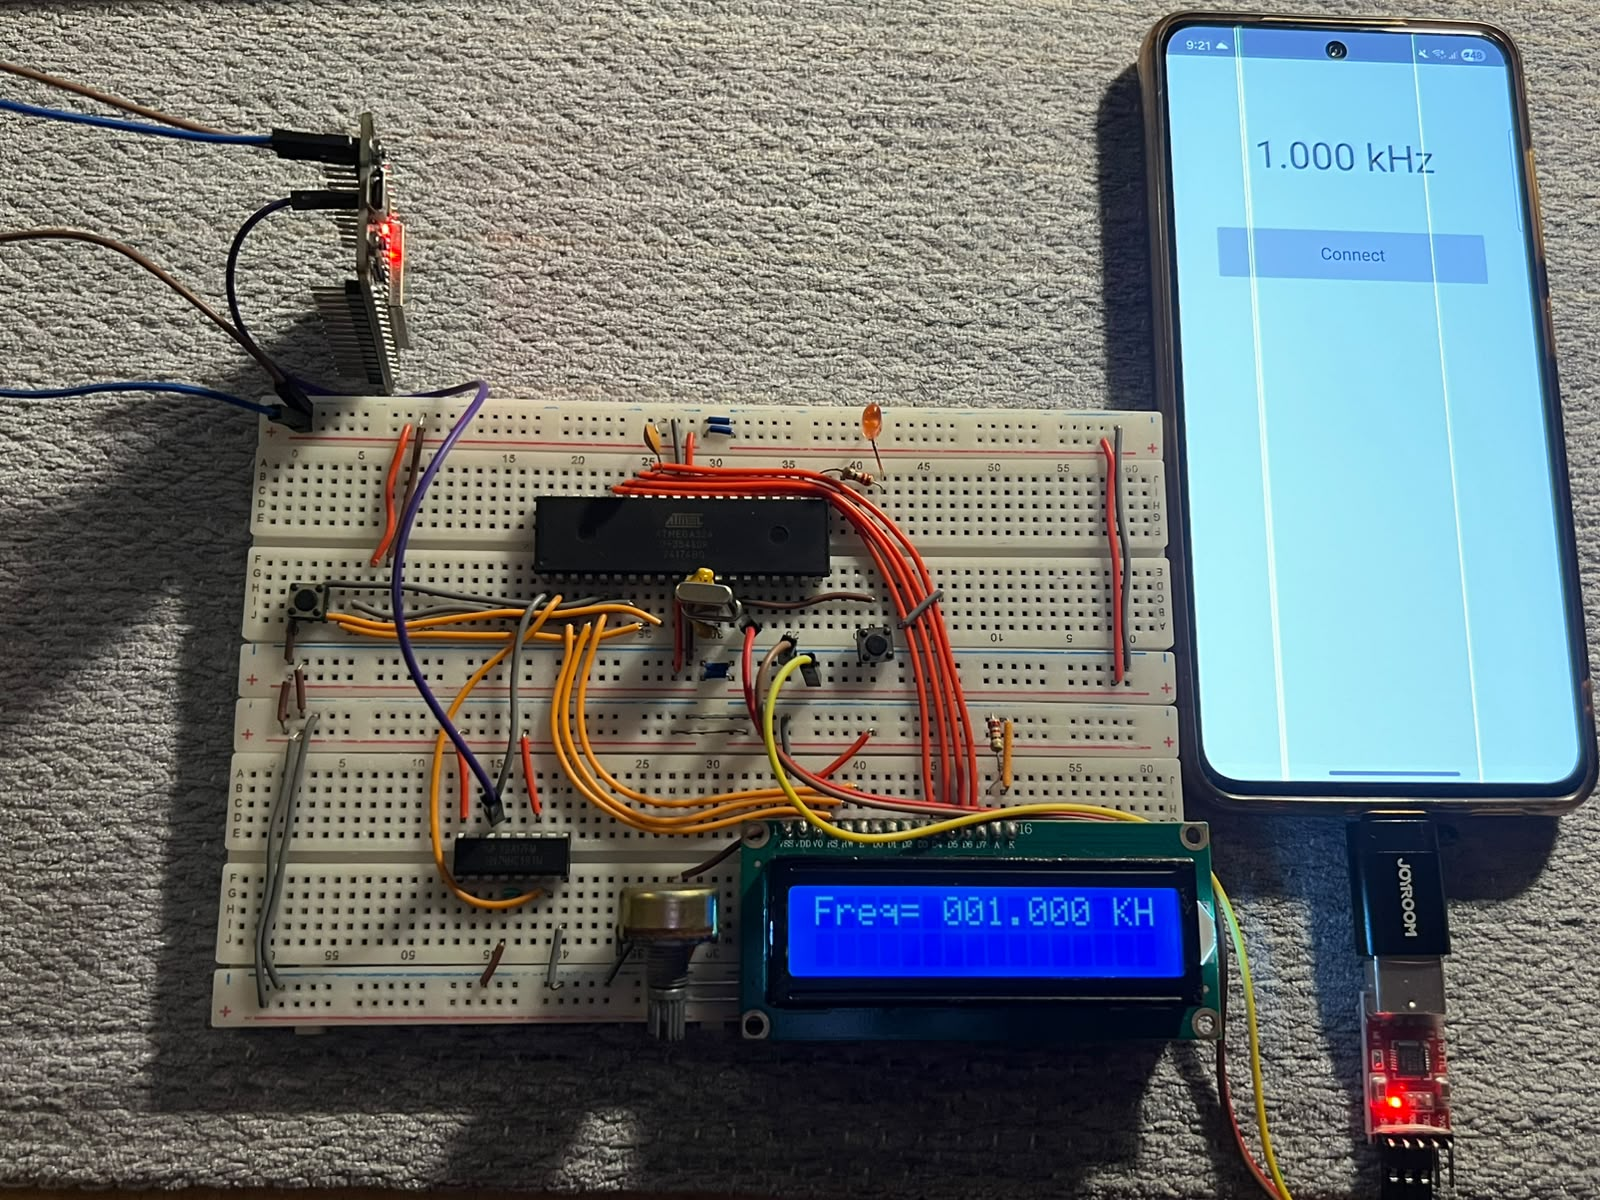
\includegraphics[width=\textwidth]{1khz_real_circuit.jpeg}
        \caption{\textbf{1\,kHz (\texttt{GPIO 25}, Direct Channel):} LCD shows \texttt{Freq= 001.000 KH}; Android app shows \texttt{1.000 kHz}.}
        \label{fig:test_1k}
    \end{subfigure}
    \hfill
    \begin{subfigure}[b]{0.485\textwidth}
        \centering
        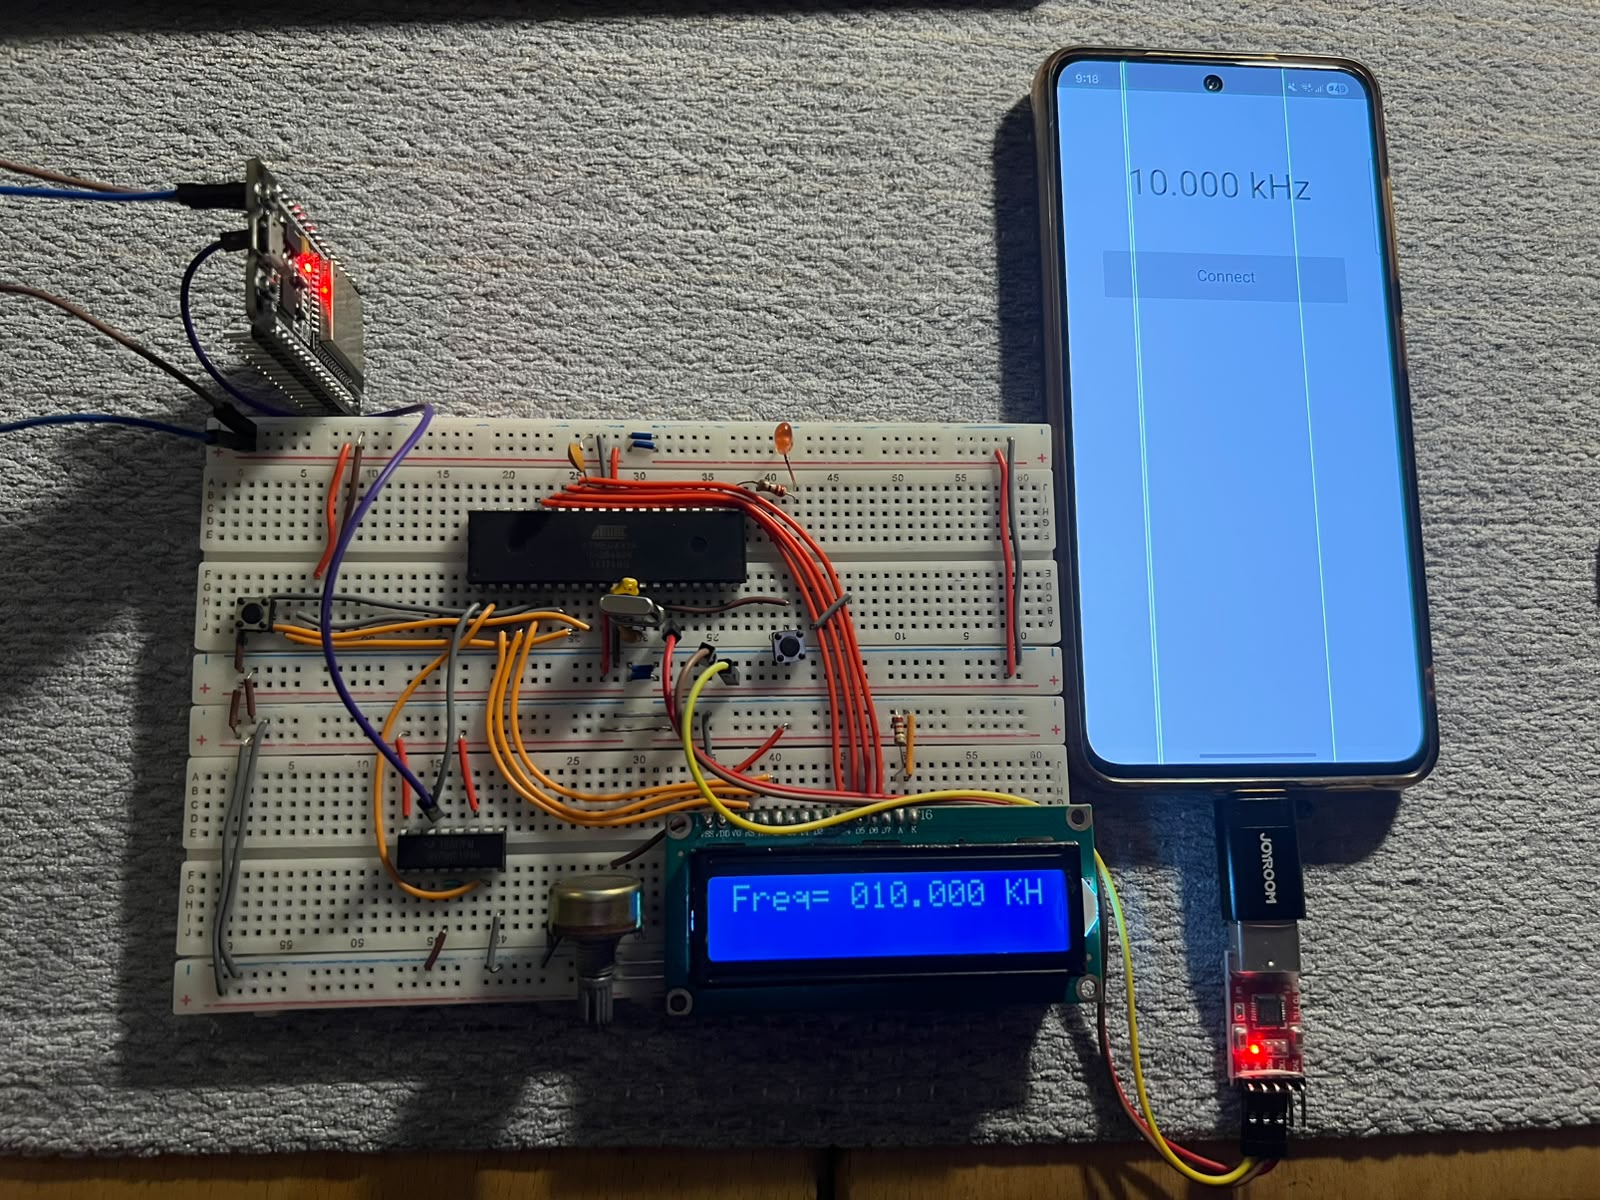
\includegraphics[width=\textwidth]{10khz_real_circuit.jpeg}
        \caption{\textbf{10\,kHz (\texttt{GPIO 26}, Direct Channel):} LCD shows \texttt{Freq= 010.000 KH}; Android app shows \texttt{10.000 kHz}.}
        \label{fig:test_10k}
    \end{subfigure}

    \vspace{0.45cm}

    \begin{subfigure}[b]{0.485\textwidth}
        \centering
        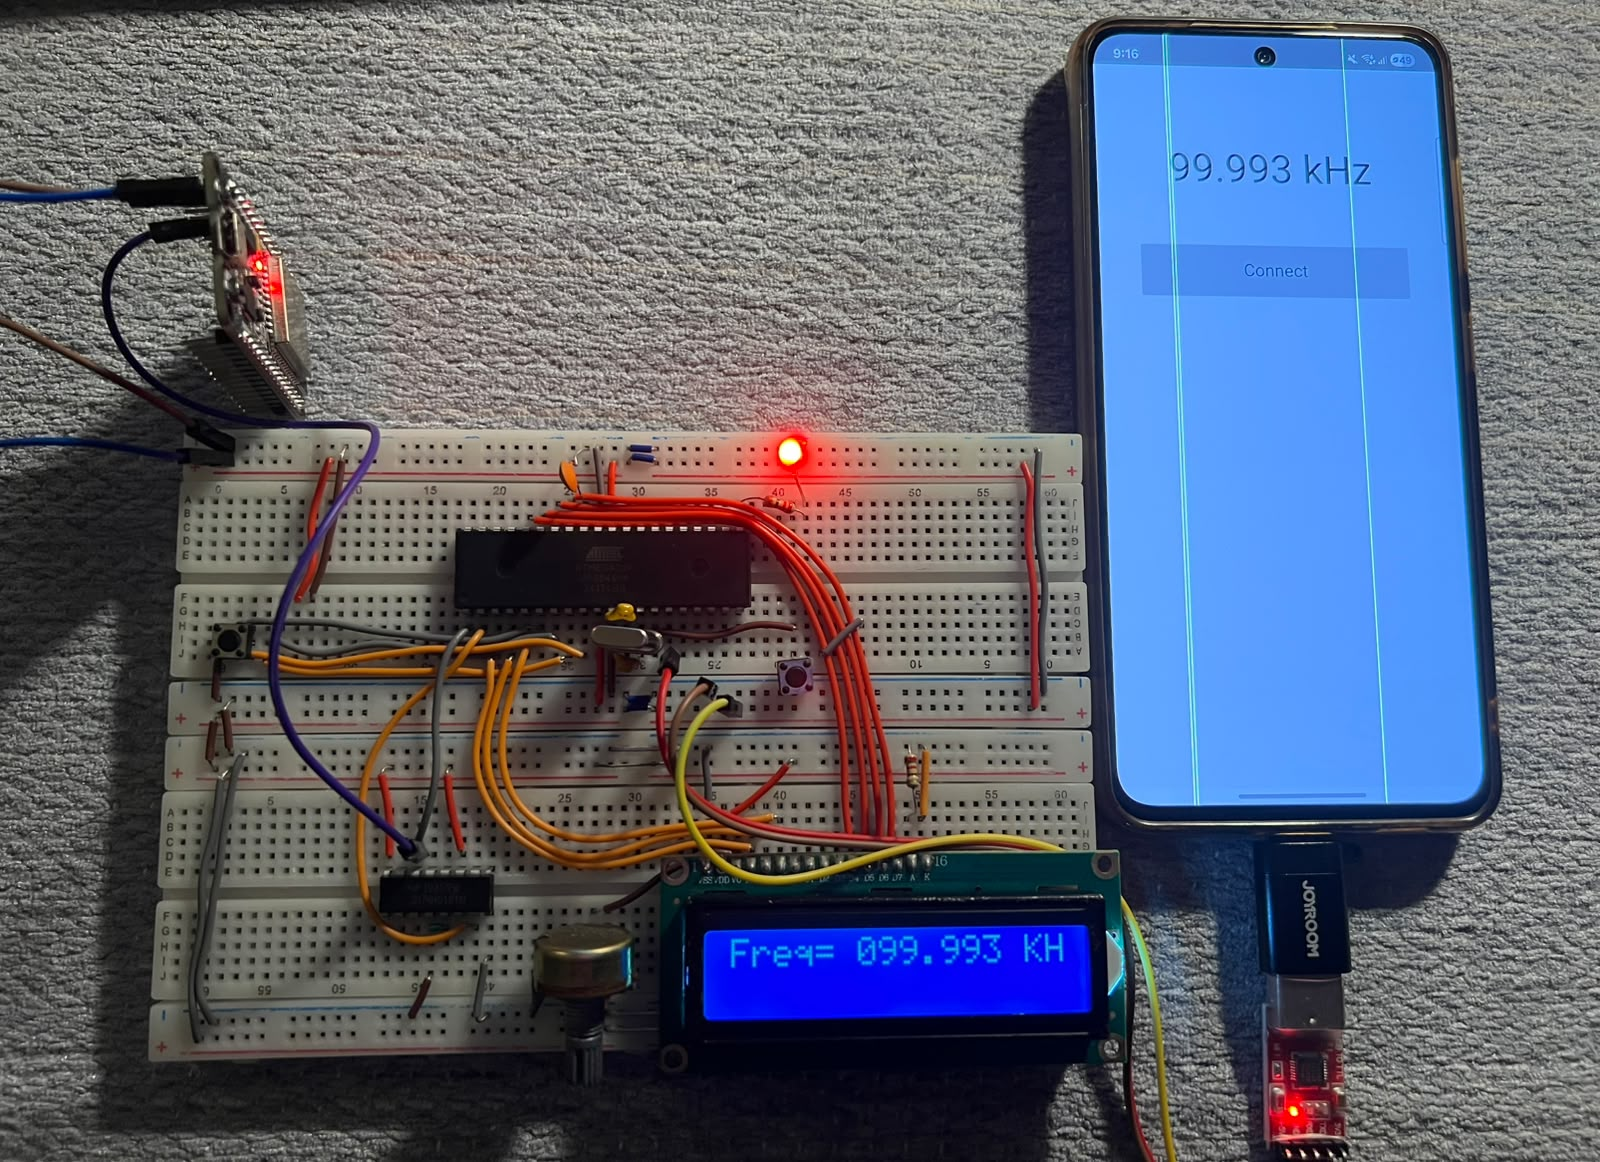
\includegraphics[width=\textwidth]{100khz_real_circui.jpeg}
        \caption{\textbf{100\,kHz (\texttt{GPIO 27}, Direct Channel):} Heartbeat LED ON; LCD shows \texttt{Freq= 099.993 KH}; Android app shows \texttt{99.993 kHz}.}
        \label{fig:test_100k}
    \end{subfigure}
    \hfill
    \begin{subfigure}[b]{0.485\textwidth}
        \centering
        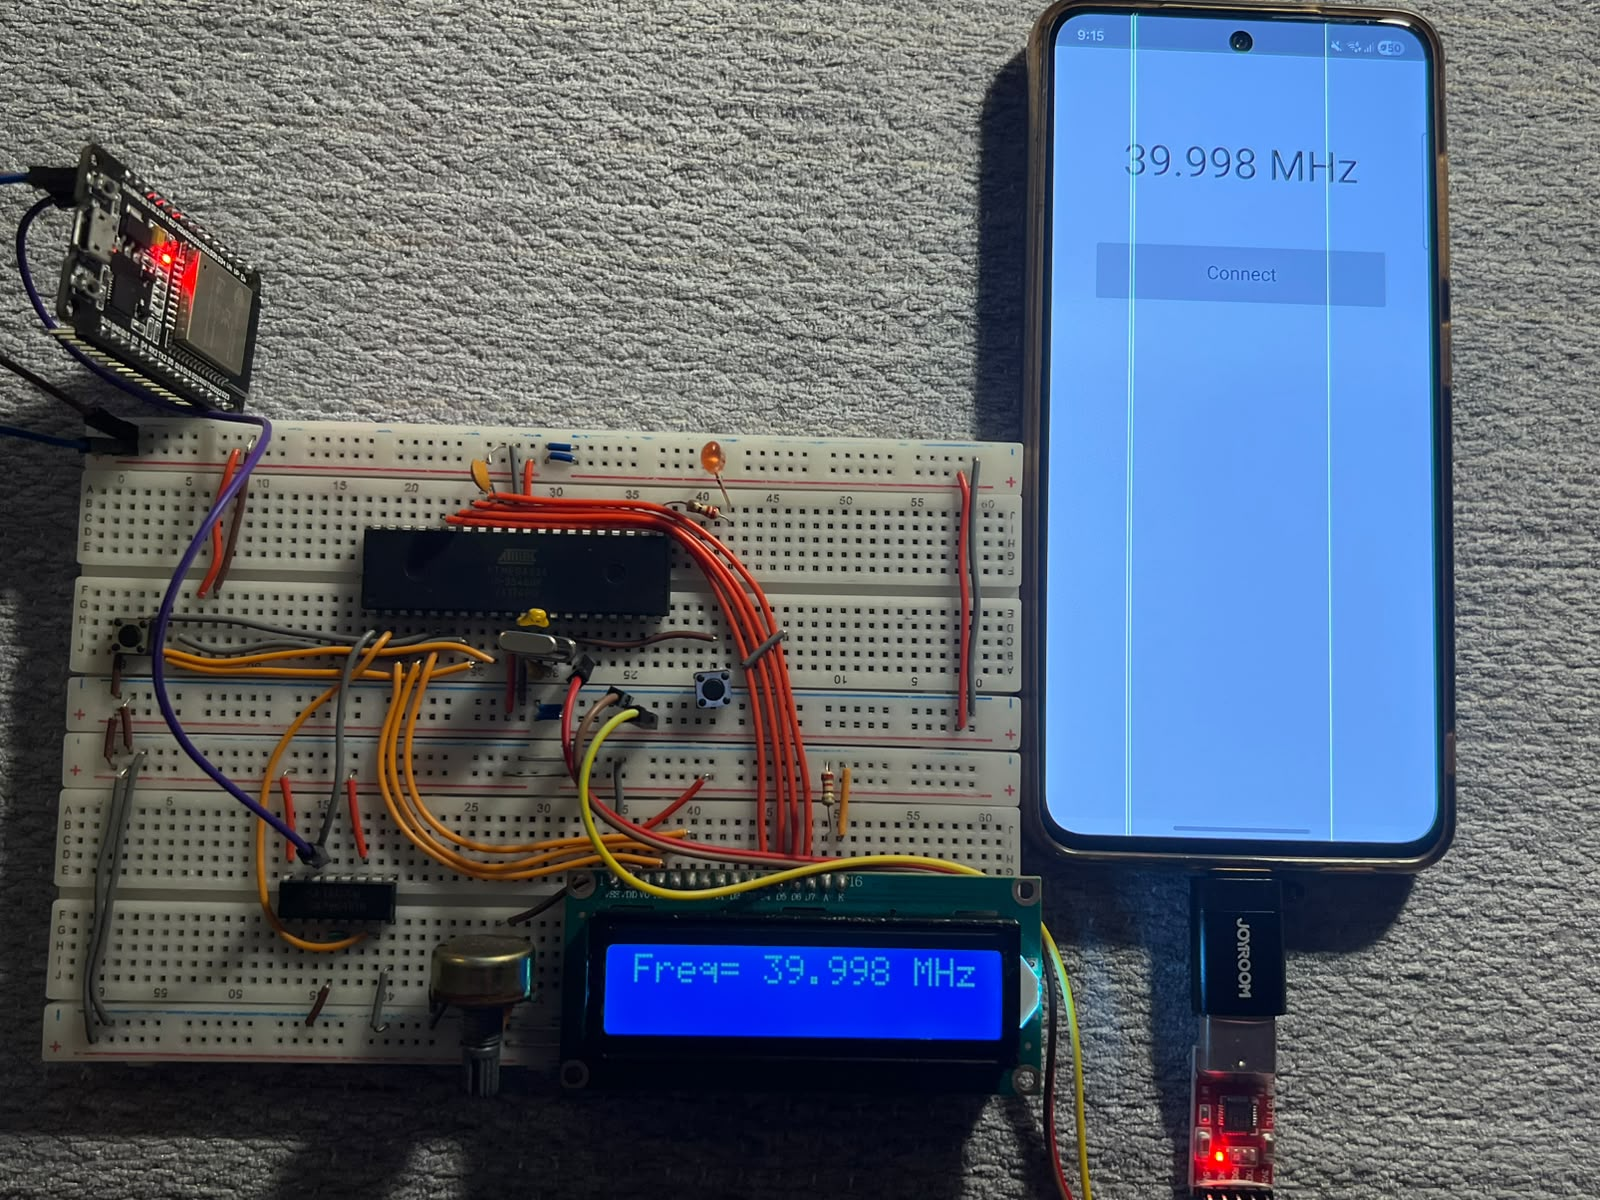
\includegraphics[width=\textwidth]{49mhz_real_circuit.jpeg}
        \caption{\textbf{40\,MHz (\texttt{GPIO 13}, Auto-Switched $\div 16$):} LCD shows \texttt{Freq= 39.998 MHz}; Android app shows \texttt{39.998 MHz}.}
        \label{fig:test_40m}
    \end{subfigure}
    \caption{Live hardware testbench results using the ESP32 pulse generator (top left), ATmega32A + 74HC191 breadboard circuit, and Android USB-OTG companion app (right) from $1\,\text{kHz}$ (\texttt{GPIO 25}) up to $40\,\text{MHz}$ (\texttt{GPIO 13}).}
    \label{fig:real_tests}
\end{figure}

\subsection{Quantitative Performance Summary}
Table~\ref{tab:results} compiles every simulated and experimental measurement together with the ESP32 source pin, active hardware channel, and calculated error.

\begin{table}[H]
\centering\small
\caption{Simulation and Experimental Measurement Accuracy}
\label{tab:results}
\renewcommand{\arraystretch}{1.2}
\begin{tabularx}{\textwidth}{X c c c c r r}
\toprule
\textbf{Test Source} & \textbf{Target} & \textbf{Channel} & \textbf{LCD Display} & \textbf{Android / UART} & \textbf{Abs. Error} & \textbf{Rel. Error} \\
\midrule
ESP32 \texttt{GPIO 25} & $1.000\,\text{kHz}$   & Direct (\texttt{T0})   & \texttt{001.000 KH} & \texttt{1.000 kHz}   & $0\,\text{Hz}$    & $0.000\%$ \\
ESP32 \texttt{GPIO 26} & $10.000\,\text{kHz}$  & Direct (\texttt{T0})   & \texttt{010.000 KH} & \texttt{10.000 kHz}  & $0\,\text{Hz}$    & $0.000\%$ \\
ESP32 \texttt{GPIO 27} & $100.000\,\text{kHz}$ & Direct (\texttt{T0})   & \texttt{099.993 KH} & \texttt{99.993 kHz}  & $-7\,\text{Hz}$   & $-0.007\%$ \\
Proteus 8 VSM          & $20.000\,\text{MHz}$  & $\div 16$ (\texttt{T1})& \texttt{19.999 MHz} & \texttt{19999920 Hz} & $-80\,\text{Hz}$  & $-0.0004\%$ \\
ESP32 \texttt{GPIO 13} & $40.000\,\text{MHz}$  & $\div 16$ (\texttt{T1})& \texttt{39.998 MHz} & \texttt{39.998 MHz}  & $-2\,\text{kHz}$  & $-0.005\%$ \\
\bottomrule
\end{tabularx}
\end{table}

\subsection{Error Analysis and Engineering Observations}
\begin{enumerate}[leftmargin=1.5em]
    \item \textbf{Crystal Tolerance and Frequency Drift ($50\text{--}70\,\text{ppm}$):}
    The small negative offsets observed at $100\,\text{kHz}$ ($-7\,\text{Hz}$, $-70\,\text{ppm}$) and $40\,\text{MHz}$ ($-2\,\text{kHz}$, $-50\,\text{ppm}$) are completely consistent with standard $\pm 30\text{--}50\,\text{ppm}$ quartz crystal tolerances on \emph{both} the ATmega32A's 11.0592\,MHz timebase and the ESP32's 40\,MHz reference crystal, plus the small CPU-cycle latency between the 43rd \texttt{Timer2} overflow ISR and halting \texttt{TCCR0}/\texttt{TCCR1B}.
    \item \textbf{Prescaler Quantization ($\pm 16\,\text{Hz}$):}
    Above $3.5\,\text{MHz}$, the 74HC191 divides the signal by 16 before reaching \texttt{Timer1}, introducing a $\pm 16\,\text{Hz}$ quantization step. At $40\,\text{MHz}$ this represents just $0.4\,\text{ppm}$ ($0.00004\%$), negligible compared to crystal accuracy.
    \item \textbf{LCD 16-Column Truncation Note:}
    Inspection of Figures~\ref{fig:test_1k}--\ref{fig:test_100k} reveals a minor cosmetic detail in \texttt{KHz()}: printing \texttt{"Freq= "} (6 chars) + \texttt{"001.000"} (7 chars) + \texttt{" KHz"} (4 chars) totals 17 characters, causing the trailing \texttt{'z'} to clip past column~16 (\texttt{Freq= 001.000 KH}). By contrast, \texttt{MHz()} fits in 16 characters (\texttt{Freq= 39.998 MHz}) and the Android app always shows the full unit (\texttt{1.000 kHz}). Shortening the LCD prefix to \texttt{"F="} or suppressing leading zeros resolves this cleanly in a single line of code.
    \item \textbf{High-Frequency Signal Integrity on Breadboard:}
    Successfully counting $40\,\text{MHz}$ on a solderless breadboard required keeping jumper wires between the ESP32 output, the 74HC191 \texttt{CLK} input, and ground short to minimize stray parasitic capacitance and ringing.
\end{enumerate}

% ============================================================================
%  SECTION 7: CONCLUSION AND FUTURE WORK
% ============================================================================
\section{Conclusion and Future Work}

\subsection{Conclusion}
We successfully designed, simulated, built, and validated a \textbf{40\,MHz dual-range auto-switching digital frequency meter} with real-time Android USB-OTG telemetry. By pairing an ATmega32A clocked at 11.0592\,MHz with a hardware 74HC191 $\div 16$ prescaler, the system bypasses the 8-bit MCU's native $\sim 4.4\,\text{MHz}$ external counting limit while retaining $1\,\text{Hz}$ precision below $3.5\,\text{MHz}$. Crystal-locked \texttt{Timer2} gating achieves an exact $1.000\,\text{s}$ timebase and $0.00\%$ UART baud-rate error simultaneously. Experimental validation using an ESP32 signal generator confirmed seamless auto-ranging and agreement between the local $16\times 2$ LCD and the Delphi FireMonkey Android app from $1\,\text{kHz}$ up to $40\,\text{MHz}$ with relative error $\le 0.007\%$.

\subsection{Future Enhancements}
\begin{itemize}[leftmargin=1.5em]
    \item \textbf{Analog Front-End Integration:} Populate the LM393 comparator snippet (\texttt{comparator.pdsclip}) with a high-impedance JFET input buffer and diode clamping so the instrument safely measures weak sinusoidal and AC analog signals (mV-level) in addition to 5\,V/3.3\,V digital clocks.
    \item \textbf{Custom 2-Layer PCB with Ground Plane:} Migrating from solderless breadboards to a dedicated PCB with a solid ground plane, short RF input traces, and an SMA/BNC input connector will reduce parasitic capacitance and push reliable operation beyond $50\,\text{MHz}$.
    \item \textbf{Reciprocal Low-Frequency Mode:} Adding an input-capture (\texttt{ICP1}) period-measurement mode below $100\,\text{Hz}$ would improve low-frequency resolution from $1\,\text{Hz}$ to $0.001\,\text{Hz}$.
    \item \textbf{Enhanced Mobile App Features:} Extending the Delphi Android app with a real-time frequency-vs.-time chart, min/max/average statistics, hold mode, and CSV export for lab logging.
    \item \textbf{LCD String Formatting Refinement:} Removing leading zeros or replacing \texttt{"Freq= "} with \texttt{"F= "} so all kHz readings display the complete \texttt{"kHz"} unit within 16 columns.
\end{itemize}

\end{document}
